\chapter{Design}
\label{chapter:design}

% \epigraph{So far, we have been able to study only one evolving system and we cannot wait for interstellar flight to provide us with a second. If we want to discover generalizations about evolving systems, we will have to look at artificial ones.}{--- \textup{John Maynard Smith}}

\minitoc[n] % minitoc without title

\section{Introduction}

  \subsection{Cooperative Robots for Collective Tasks}

    Multi-robots systems (MRS) essentially gained fame during 1980s under the idea of trying to cope with tasks that classical single robots sometimes could not. MRS can basically be constitued of between two to a thousand robots~\cite{Rubenstein2014} depending on the task at hand. While it may seem counter-productive to develop and control several robots where a single robot could very well achieve the task, using a team of robots has several advantages among which~\cite{Cao1997, Arkin1998}:

    \begin{itemize}
      \item{The parallel execution of multiple robots allow the task to be achieved faster.}
      \item{Several robots can ensure robustness through \emph{redundancy}.}
      \item{It can be both cheaper and simpler to produce several simple robots that a single complex one (especially if the robot is expected to suffer destruction).}
      \item{It may be necessary to distribute several robots at the same time to achieve the task, in which case a single robot could obviously not.}
    \end{itemize}

    -> Parler de CEBOT et Herd Nerd qui sont un peu les premiers (Parker1994)

    -> Heterogeneous VS Homogeneous, decentralized VS centralized: control architecture

    -> Biological inspiration (Cao) == Swarm ?

    -> Swarm

    -> self-organization

    -> DAI



  \subsection{Designing Collective Robots}
    \begin{itemize}
      \item{General (quick) review on the design of collective robots without ER}
      \item{Should obviously highlight the advantages of using ER}
    \end{itemize}

  \subsection{Evolving Cooperation}
    \begin{itemize}
      \item{Review of the works in ER where cooperation is evolved and where we stand in this context (and why)}
    \end{itemize}












































\section{Evolution of Cooperation in Evolutionary Robotics: the Tradeoff between Evolvability and Efficiency}

  \subsection{Introduction}

  The evolution of cooperative actions in evolutionary robotics is as much a challenge as an interesting perspective for the design of complex collective systems~\cite{Doncieux2015}. As such, it has been widely studied with very diverse approaches and objectives~\cite{Waibel2009, Hauert2014, Trianni2007, Lichocki2012}. These works often use a clonal paradigm, where each robot has a copy of the same genome. This makes sense as this is the easiest way to ensure cooperation when individuals are expected to display similar behaviors. Moreover, using clones ensures minimal genetic relatedness between individuals, which is known to allow the evolution of altruism~\cite{Waibel2011, Montanier2011}. As such, most research focus on increasing the probability for the cooperative solution to evolve.

  In comparison, the nature of coordination behaviors and their influence on the quality of cooperation has yet to be thoroughly studied. In particular, interactions between clones in evolutionary robotics tend to produce homogeneous behaviors when most coordination tasks could benefit from heterogeneous behaviors. This could be solved by using a non-clonal approach where paired individuals do not use the same genome, and could possibly evolve different behaviors more easily. However, a non-clonal approach may face a \emph{chicken-and-egg} dilemma: multiple individuals need to behave in a particular fashion for cooperation to be rewarding, but no benefit can be extracted from this behavior unless all individuals cooperate. Therefore, without cooperating partners, those behaviors cannot be selected by the evolution as they do not benefit the individual. This is particularly problematic when a moderately rewarding solitary strategy overshadows a more rewarding, but also more challenging to evolve, cooperative strategy~\cite{Skyrms2004}.

  In this paper, we are interested in the comparison between clonal and non-clonal approaches on two different criteria:
 \begin{itemize}
    \item{\emph{Evolvability} of cooperation, which is the number of successful runs where cooperation evolved.}
    \item{\emph{Efficiency} of cooperation. This criteria is focused on the quality of the evolved behaviors and is determined by the   performance (w.r.t. fitness score) of the coordination strategies.}
  \end{itemize}

  To that end, we design a foraging task where both cooperative and solitary strategies are possible but where cooperation provides the largest reward. This task is favored by the evolution of efficient cooperative behaviors and we compare different approaches on both criteria. The first approach is a straightforward implementation of the literature where interacting individuals are clones. In comparison, the second approach is a rather extreme implementation of a non-clonal approach: we use coevolution, where individuals are from two different populations, and where fitness scores are computed independently for each individual. While this scheme is typical of competitive coevolution~\cite{Floreano1997, Floreano1998,Panait2005}, the nature of the task considered here makes cooperation more interesting, as both individuals can selfishly benefit from being cooperative.

  In the next section, we describehe methods and experimental setup used throughout our study. Then, we compare the results of the two approaches on the cooperative task. This first experiment reveals that both approaches face a tradeoff between evolvability and efficiency, where neither one dominates the other on both criteria. We investigate in a second experiment the possibility to overcome this tradeoff for both approache s. To this end, we use incremental evolution~\cite{Harvey1994, Urzelai1998} and evolve coordination in a simpler task in order to improve both the evolvability and efficiency on the target task for each approach. Finally, we discuss the implication of our findings in the last section, in particular with respect to maximizing evolvability and efficiency alike.


  \subsection{Methods}
  

  Two robotic agents are placed in a 800 by 800 units square arena with four solid walls and emptied from any obstacle apart from the targets in the foraging task. Each circular-shaped agent, with a diameter of 20 units, has a collection of sensors divided between a 90 degrees front camera and 12 uniformly distributed proximity sensors. The camera is composed of 12 rays with infinite range which indicate the type (coded on 3 bits) and proximity (one value in $R^n$) of the nearest object or agent in their direction. Proximity sensors have a range of twice the agent body's diameter and are used to get the distance to any obstacle nearby such as solid objects, the other agent or walls. The two agents always begin the simulation next to one another at one end of the arena, whereas all the objects' initial positions are randomized.

  Agents can move freely in the environment and are controlled by a fully connected multi-layer perceptron with a single hidden layer, the topology of which does not change during the evolution. Inputs of this neural network are fed with all the data extracted from the sensors: 48 neurons for the camera (4 neurons for each of the 12 rays) and 12 neurons for the proximity sensors. A bias neuron, whose value is always 1, brings the total number of input neurons to 61. The hidden layer is comprised of 8 neurons and the output layer of 2 neurons giving the speed of each of the agent's wheels. The activation function used is a sigmoid.

  In each experiment, individuals evolved during a fixed amount of evaluations thanks to an evolutionary algorithm. Their genome consists of a collection of the 506 connection weights (as real-values) of the neural network and is initially randomized for each individual in the population. Three evaluation setups are used to compare the different approaches of our experiment: 

  \begin{itemize}
    \item{In the \emph{control} setup, each individual is evaluated against 5 other randomly chosen individuals in the population except itself. Therefore we ensure that there is no genetic relatedness between individuals in each pair. However, it is not clear how the evolutionary algorithm itself may impact the population's diversity, especially because elitism is used;}
    \item{In the \emph{clonal} setup, each individual is evaluated once against a clone of itself. This setup is used to study the results of the classical clonal approach~\cite{Waibel2009, Hauert2014, Trianni2007, Lichocki2012}. While previous works have shown on multiple occasions that cooperation can evolve, it is not clear if individuals can take different roles during a cooperative interaction;}
    \item{In the \emph{coevolution} setup, each ofhe two individuals comes from two different coevolved populations. In this setup, each individual from one population encounters 5 random individuals from the other population. As pairing considers individuals from two seperate populations, the evolution of heterogeneous behaviors is theoretically easier. As a matter of fact, such a relation where two very different individuals find a selfish   interest in mutual cooperation is actually quite common in nature~\cite{Connor1995}.}
  \end{itemize}
 A pair of individuals then interact in the arena described before for a fixed number of simulation steps called a trial. Each trial is conducted $5$ times to account for the random initial positions of the objects and decrease the influence of the initial conditions on the individuals' performance. 
  
  The selection method used in the evolutionary algorithm is an elitist (10+10)-ES where the 10 best individuals in the population are used to generate 10 offsprings for the next generation. We use no recombination and therefore each offspring is a mutated copy of its parent. Mutations were sampled according to a gaussian operator with a standard deviation of \(1.10^{-2}\) and a gene's mutation rate of \(5.10^{-3}\). Finally, population size was kept constant through the evolution with a number of $20$ individuals. All experiments were done using the framework for evolutionary computation SFERESv2~\cite{Mouret2010}, which includes a fast 2D robotic simulator. The source code for reproducing the experiments is available for download at http://pages.isir.upmc.fr/\textasciitilde bredeche/Experiments/ECAL2015-coop.tgz.


  \subsection{Cooperative Foraging Task}
  
  In this first experiment, we investigate the evolution of cooperation in a foraging task. The environment is filled with 18 solid targets that the agents can collect. To collect a target, an agent has to stay close to this object for a fixed amount of simulation steps (800). After this duration, the target disappears and any agent close to it is rewarded with its value. Targets are of two types. Green targets always reward 50 when collected whereas purple ones reward 250 only when the agents collect it together (Table~\ref{tab:Rewards}). If a solitary agent collects a purple target, it disappears and rewards nothing. Consequently, there is both an incentive and a risk to cooperate as cooperation is dependent on successful coordination. This setup is a robotic implementation of a well-known problem in game theory for studying the evolution of mutualistic cooperation: the {\em Stag Hunt}~\cite{Skyrms2004}.

  The fitness score (\(F\)) of an individual is the average reward per trial:
 \[
  F = \frac{1}{N*M} \sum_{i=1}^{N} \sum_{j=1}^{M} f_{ij}
  \]
  
  Where \(N\) is the number of individuals encountered ($5$ in the control and coevolution setups, $1$ in the clonal setup), \(M\) the number of trials ($5$) and \(f_{ij}\) the rewards obtained at trial \(j\) with individual \(i\).

  When a target is collected, another target of the same type is then placed at a random position in the arena to keep a constant ratio between green and purple targets. Each evaluation lasted 20000 simulation steps and 60 independent runs were conducted for each experimental setup, each one lasting 40000 evaluations.

  \begin{table}[hbtp]
    \center{
      \begin{tabular}{lrc}
        \hline
        \multicolumn{2}{l}{\textbf{Target}} & \textbf{Reward} \\
        \hline
        Green & & \\
        & \textit{alone} & 50 \\
        & \textit{coop} & 50 \\
        Purple & & \\
        & \textit{alone} & 0 \\
        & \textit{coop} & 250 \\
        \hline
      \end{tabular}
    }
    \caption{Rewards for the foraging of the different targets, depending on whether they were collected alone or cooperatively.}
    \label{tab:Rewards}
  \end{table}

  \subsubsection{Results}

  \begin{table}[hbtp]
    \center{
      \begin{tabular}{lccc}
        \hline
        \textbf{Setting} & \textbf{\# Coop.} & \textbf{\# Solitary} & \textbf{Total}\\ 
        \hline
        \textit{Control} & 10 & 50 & \textbf{60}\\
        \textit{Clonal} & 28 & 32 & \textbf{60}\\
        \textit{Coevolution} & 14 & 46 & \textbf{60}\\
        \hline
      \end{tabular}
    }
    \caption{Number of simulations where the best individual evolved a cooperative strategy (collecting purple targets) or a solitary strategy (collecting green targets) for each setup in the foraging task.}
    \label{tab:ForagingCoop}
  \end{table}

  We are interested in the number of simulations where cooperation evolved (i.e. the \emph{evolvability} of each approach), which means simulations where the best individual in the population evolved the cooperative foraging of the purple targets (i.e. more than $50$\% of the collected targets are purple). Results for the three setups are displayed in Table~\ref{tab:ForagingCoop}. As could be expected from the literature, the clonal setup displays a greater evolvability w.r.t. evolving cooperation (28/60), whereas coevolution (14/60) is on par with the control setup (10/60). It is also apparent that cooperation is still difficult to evolve as in the best case (clonal), no more than half the simulations display the evolution of cooperative behaviors.

  \begin{figure}[hbtp]
    \begin{center}
      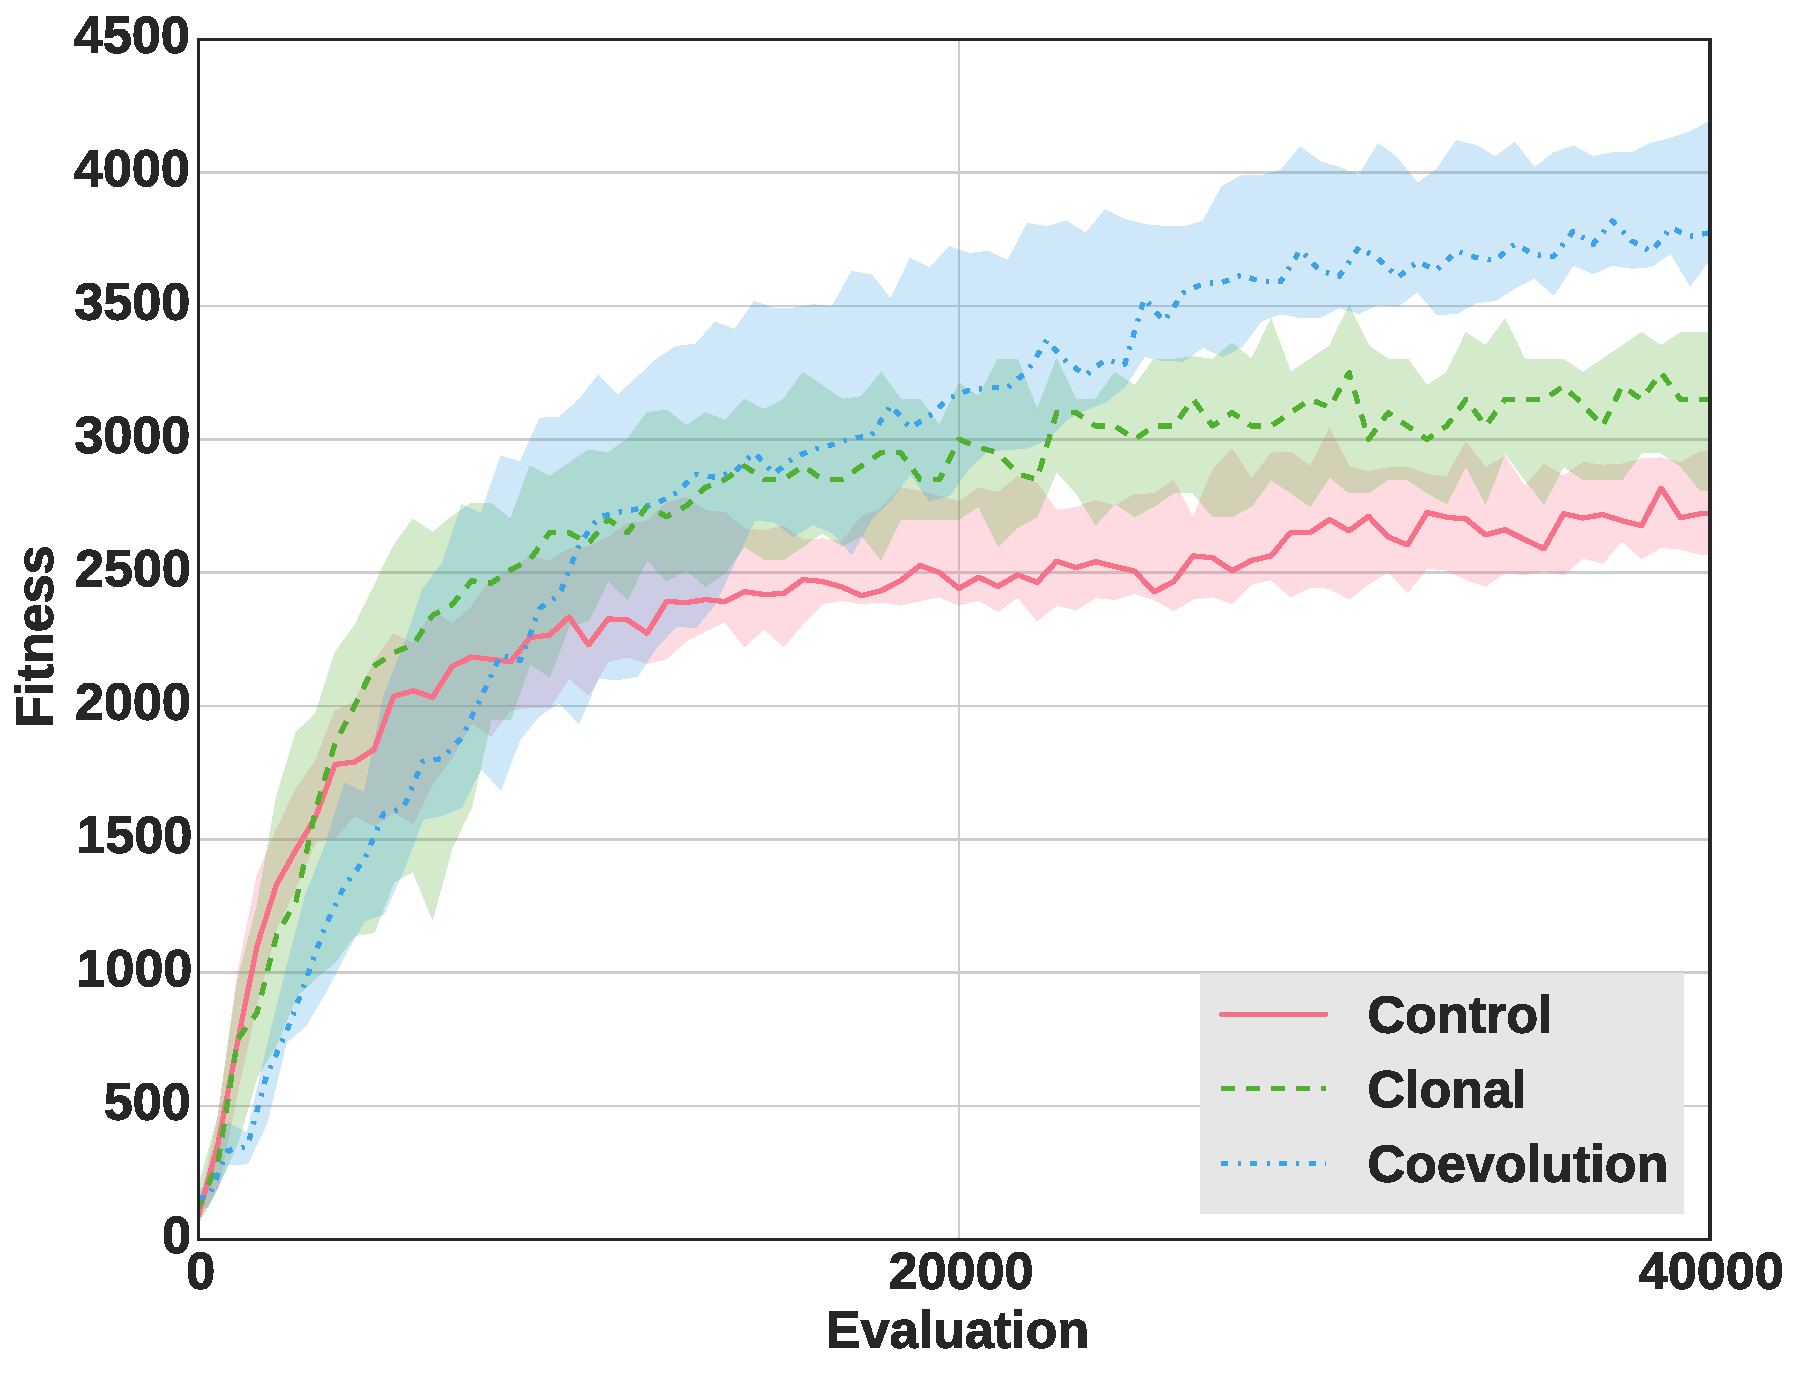
\includegraphics[scale = 0.30]{fig/ArticleRob1/fitnessHuntingStags.pdf}
      \caption{Median fitness score of the best individuals in each of the runs where cooperation evolved for each setup over time. The fitness score of an individual is computed as the average reward the individual earned per trial by foraging targets. The colored areas around the medians represent the first and third quartiles.} 
      \label{fig:HuntingFitness}
    \end{center}
  \end{figure}

  However, cooperative individuals do not perform with the same \emph{efficiency} from one setup to another. We show in Figure~\ref{fig:HuntingFitness} the median fitness score of the best individuals in each independent run where cooperation evolved over time and for each setup. Fitness scores are significantly different in each setup with the best score obtained in the coevolution setup and the worst in the control setup (Mann-Whitney U-test on the fitness score of the best individuals at the last evaluation, {\em p}-value $< 0.001$).

  These differences in efficiency can be explained by looking at the nature of the cooperative behaviors evolved, which reveals two types of behaviors: \emph{turning} and \emph{leader/follower}.

  Individuals adopting the turning strategy turn around one another so that they always see the other individual as well as stay close to it (Figure~\ref{fig:behaviorHuntingTurning}). This allows the two individuals to approach simultaneously a same target and therefore forage it in a cooperative fashion. In this strategy, both individuals have a similar behavior and no role division is necessary for their successful cooperation.

  In comparison, individuals which evolve a leader/follower strategy adopt a differentiation between two roles: \emph{leader} and \emph{follower} (Figure~\ref{fig:behaviorHuntingLeadership}). The individual we call leader always goes first on a target whereas the follower always arrives second on the same target. We observe that the follower's behavior consists in staying close to the leader and always keeping it in front of itself. In comparison the leader shows a lesser interest in the presence of its follower and rarely checks on its position.


  \begin{figure}[hbtp]
    \centering
      \begin{subfigure}[]
        {\label{fig:behaviorHuntingTurning} 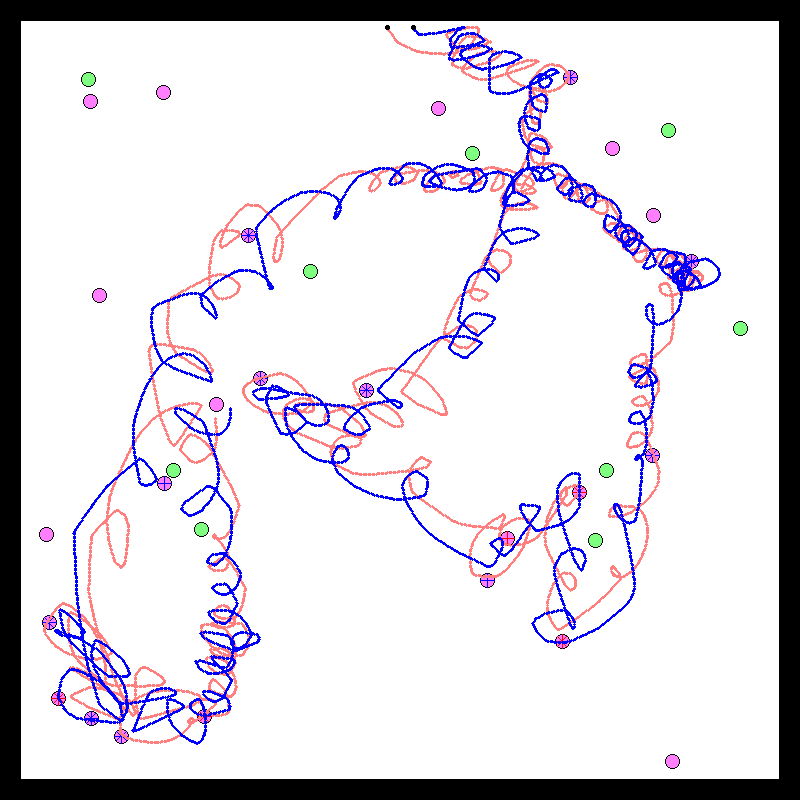
\includegraphics[scale=0.25]{fig/ArticleRob1/behaviorHuntingTurning.png}}
      \end{subfigure}~
      \begin{subfigure}[]
        {\label{fig:behaviorHuntingLeadership} 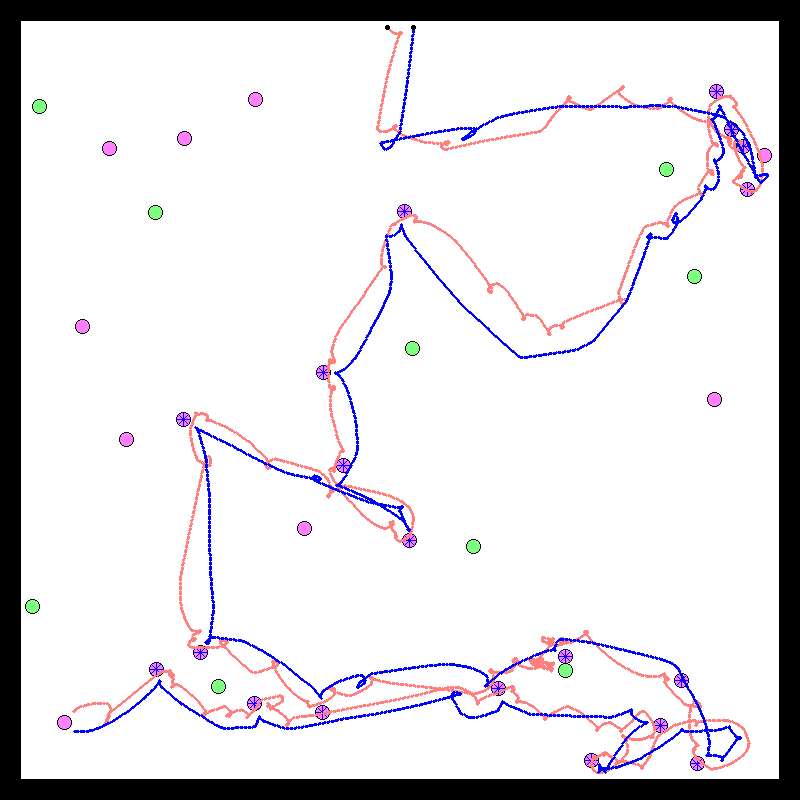
\includegraphics[scale=0.25]{fig/ArticleRob1/behaviorHuntingLeadership.png}}
      \end{subfigure}
      \caption{Snapshots of the simulation after an entire trial in the foraging task. The path of each robotic agent from their initial positions (black dots) is represented in red and blue. The green and purple discs represent the 18 targets in the environment. When a target is foraged by the two agents, a red cross (resp. blue) is drawn on the target if the red agent (resp. blue) arrived on it first. Each snapshot corresponds to a trial where agents adopted a different behavior: {\em (a)}~turning or {\em (b)}~leader/follower.}
      \label{fig:behaviorTracesHunting}
  \end{figure}


  Table~\ref{tab:ForagingBehaviors} shows the distribution of cooperative strategies for all three setups. Whereas the control and clonal setups always resulted in turning strategies (resp. 10/10 and 28/28), the coevolution setup always displayed the evolution of a leader/follower strategy (14). We observe that this latter strategy leads to more efficient cooperation. Indeed, individuals adopting the turning strategy are forced to check constantly on the other individual's position. Consequently, they cannot be as fast as individuals with a leader/follower strategy where they move to the target in a straight line under the leader's direction. Moreover, due to the random proximity of the targets, the turning strategy is prone to errors. Namely, they often get to another target than that of their partner whenever two targets are too close to each other.

  A possible explanation as to why no leader/follower strategy could evolve in the control and clonal setups may be because of the need to differentiate between the two roles. Indeed, there needs to be the existence of an asymmetry between the two individuals for this phenomenon to appear. With coevolved populations, this asymmetry is deliberately created by the separation between the two populations. Indeed, we observe that one population exclusively contains leaders while the other exclusively contains followers. 

  The two other setups fail to evolve heterogeneous behaviors. In the control setup, this may be due to the evolutionary algorithm used, especially with elistism enforcing the homogenization of the population throughout the course of evolution (as hinted in the Methods Section). Then, the clonal setup introduces yet another challenge as switching to a particular role can only be done during evaluation as both individuals are by definition genetically similar.

  \begin{table}[hbtp]
    \center{
      \begin{tabular}{lccc}
        \hline
        \textbf{Setting} & \textbf{\# Leader/Follower} & \textbf{\# Turning} & \textbf{Total}\\ 
         & \textbf{Strategy} & \textbf{Strategy} & \\ 
        \hline
        \textit{Control} & 0 & 10 & \textbf{10}\\
        \textit{Clonal} & 0 & 28 & \textbf{28}\\
        \textit{Coevolution} & 14 & 0 & \textbf{14}\\
        \hline
      \end{tabular}
    }
    \caption{Repartition of the different strategies evolved in each of the runs where cooperation evolved for each setup in the foraging task. We indicate in each cell the number of simulations where a particular strategy evolved.}
    \label{tab:ForagingBehaviors}
  \end{table}

  \subsection{Going Beyond the Evolvability vs. Efficiency Tradeoff using Incremental Evolution}

  The previous section revealed a tradeoff between evolvability and efficiency. In the clonal setup, cooperation evolves more often than with other setups. However, the coevolution setup yields cooperative behaviors which are more efficient, with paired individuals displaying asymmetrical behaviors.

  In this section, we address the following question: is it possible to benefit from both evolvability \textit{and} efficiency with the clonal and/or the coevolution setups? In other words, we explore (1) whether the clonal setup can be used to evolve pairs with heterogeneous behaviors, and (2) whether the coevolution setup can be improved in terms of number of runs where cooperation evolved.

  In order to address this question, we use incremental evolution, a rather common method in evolutionary robotics for solving challenging problems~\cite{Dorigo1994,Saksida1997,Bongard2008,Doncieux2013}. The main principle is to ease the learning of a complex task by splitting it into simpler sub-tasks~\cite{Perkins1996}.

  In the following, we introce an additional task, the \textit{waypoints crossing} task, which requires the evolution of coordination behaviors, and is simpler to address than the preous task. Individuals evolved in this first task are then used as starting point for the original task described earlier, hoping that cooperative behavior will be \emph{recycled} from the first task to the second task.
  
  \subsubsection{Waypoints Crossing Task}  

  We consider a task where robotic agents have to cross randomly positioned waypoints. As such, these round waypoints do not act as obstacles and have a diameter of 30 units. As soon as an agent goes through a waypoint, it can not be seen by this agent anymore. All 18 waypoints have the same color and can be crossed in any order. The fitness score (\(F\)) of each individual is defined as the average longest sequence of waypoints shared by both agents per trial:

  \[
  F = \frac{1}{N*M} \sum_{i=1}^{N} \sum_{j=1}^{M} l_{max_{ij}}
  \]

  Where \(N\) is the number of individuals encountered ($5$ in the control and coevolution setups, $1$ in the clonal setup), \(M\) the number of trials ($5$) and \(l_{max_{ij}}\) the longest sequence of waypoints shared by both individuals at trial \(j\) with individual \(i\).

  This implies that the two individuals are rewarded when crossing waypoints in the same order as well as maximizing the number of waypoints crossed. Each evaluation lasted $10000$ simulation steps and $60$ independent runs were conducted for each experimental setup, each one lasting $40000$ evaluations.

  \begin{figure}[hbtp]
    \begin{center}
      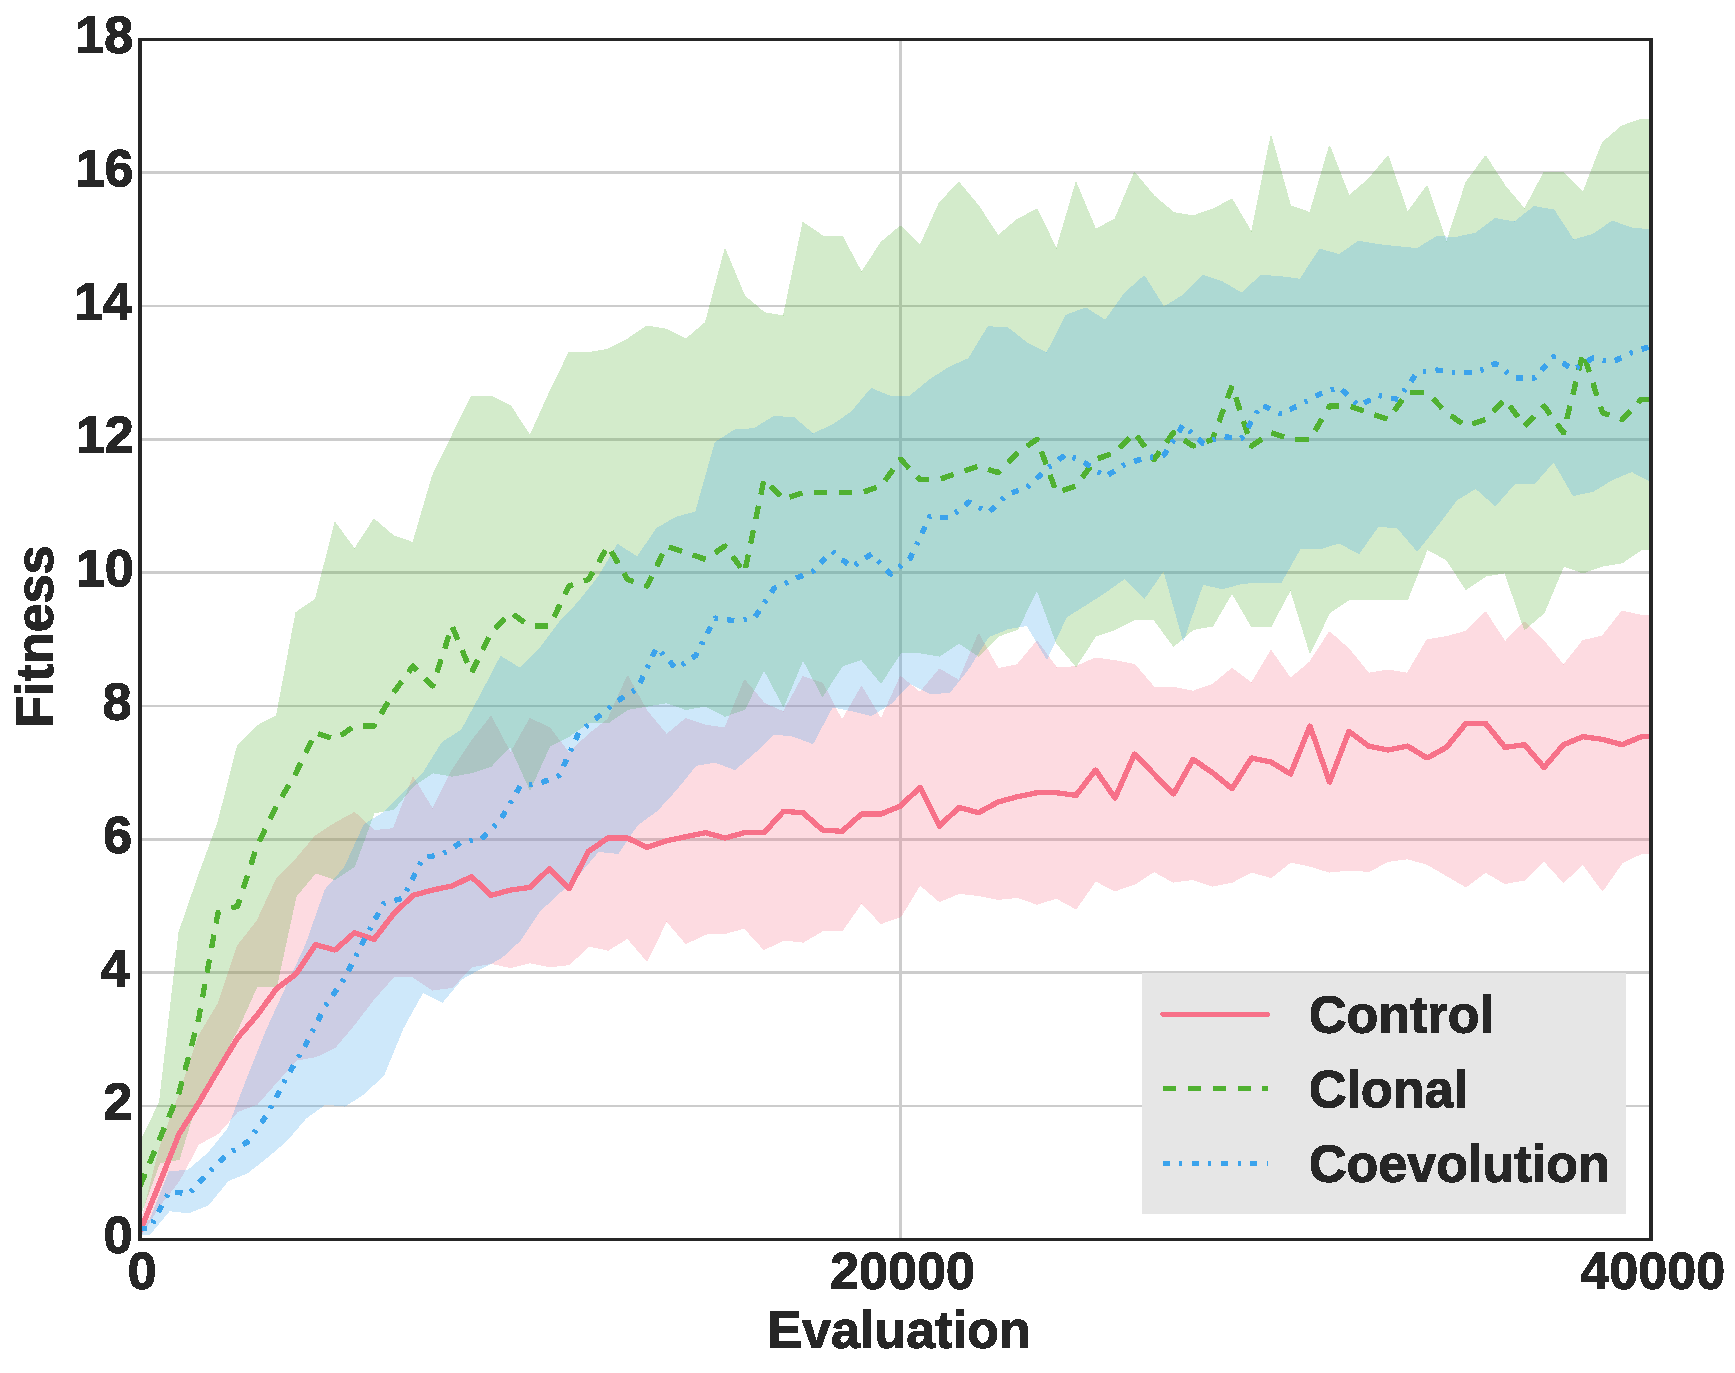
\includegraphics[scale = 0.3]{fig/ArticleRob1/fitnessWaypoints.pdf}
      \caption{Median fitness score of the best individuals in each of the 60 independent runs and for each setup over time. Fitness score is computed as the average longest sequence of waypoints shared by both agents per trial. The colored areas around the medians represent the first and third quartiles.}
      \label{fig:WaypointsFitness}
    \end{center}
  \end{figure}

  All simulations showed an increase in fitness score for each of the three setups (cf. Figure~\ref{fig:WaypointsFitness}). This was expected as this task does not represent a particular challenge for the individuals: it simply needs the evolution of a successful coordination strategy. However, whereas the coevolution and clonal setups performed equally, they both surpassed the performance of individuals from the control setup (Mann-Whitney, {\em p}-value $< 0.001$).

  As with the previous foraging task, we can hypothesize that these differences in fitness scores are due to differences in the behaviors evolved. Table~\ref{tab:WaypointsBehaviors} gives a classification of the cooperative behaviors for each setup. They are similar to those in the previous task with the addition of a third rare strategy: the \emph{wall-following} strategy (which is regrouped in ``Other''). Wall-followers simply follow the walls around the arena and cross any waypoints close to the wall they are adjacent to. As such, this is a far less efficient strategy than the two others. 


  \begin{table}[hbtp]
    \center{
      \begin{tabular}{lcccc}
        \hline
        \textbf{Setting} & \textbf{\# Lead.} & \textbf{\# Turn.} & \textbf{\# Other} & \textbf{Total}\\ 
         % & \textbf{Strategy} & \textbf{Strategy} & \textbf{Strategy} & \\ 
        \hline
        \textit{Control} & 19 & 37 & 4 & \textbf{60}\\
        \textit{Clonal} & 23 & 31 & 6 & \textbf{60}\\
        \textit{Coevolution} & 59 & 1 & 0 & \textbf{60}\\
        \hline
      \end{tabular}
    }
    \caption{Repartition of the different strategies evolved in each of the 60 independent runs for each setup in the waypoints task. We indicate in each cell the number of simulations where a particular strategy evolved: \emph{Leader/follower} (Lead.), \emph{Turning} (Turn.) or \emph{Other}. ``Other'' regroups wall-following strategies or simulations where no recognizable strategy evolved.}
    \label{tab:WaypointsBehaviors}
  \end{table}

  \begin{figure}[hbtp]
    \centering
      \begin{subfigure}[]
        {\label{fig:leadershipControl} 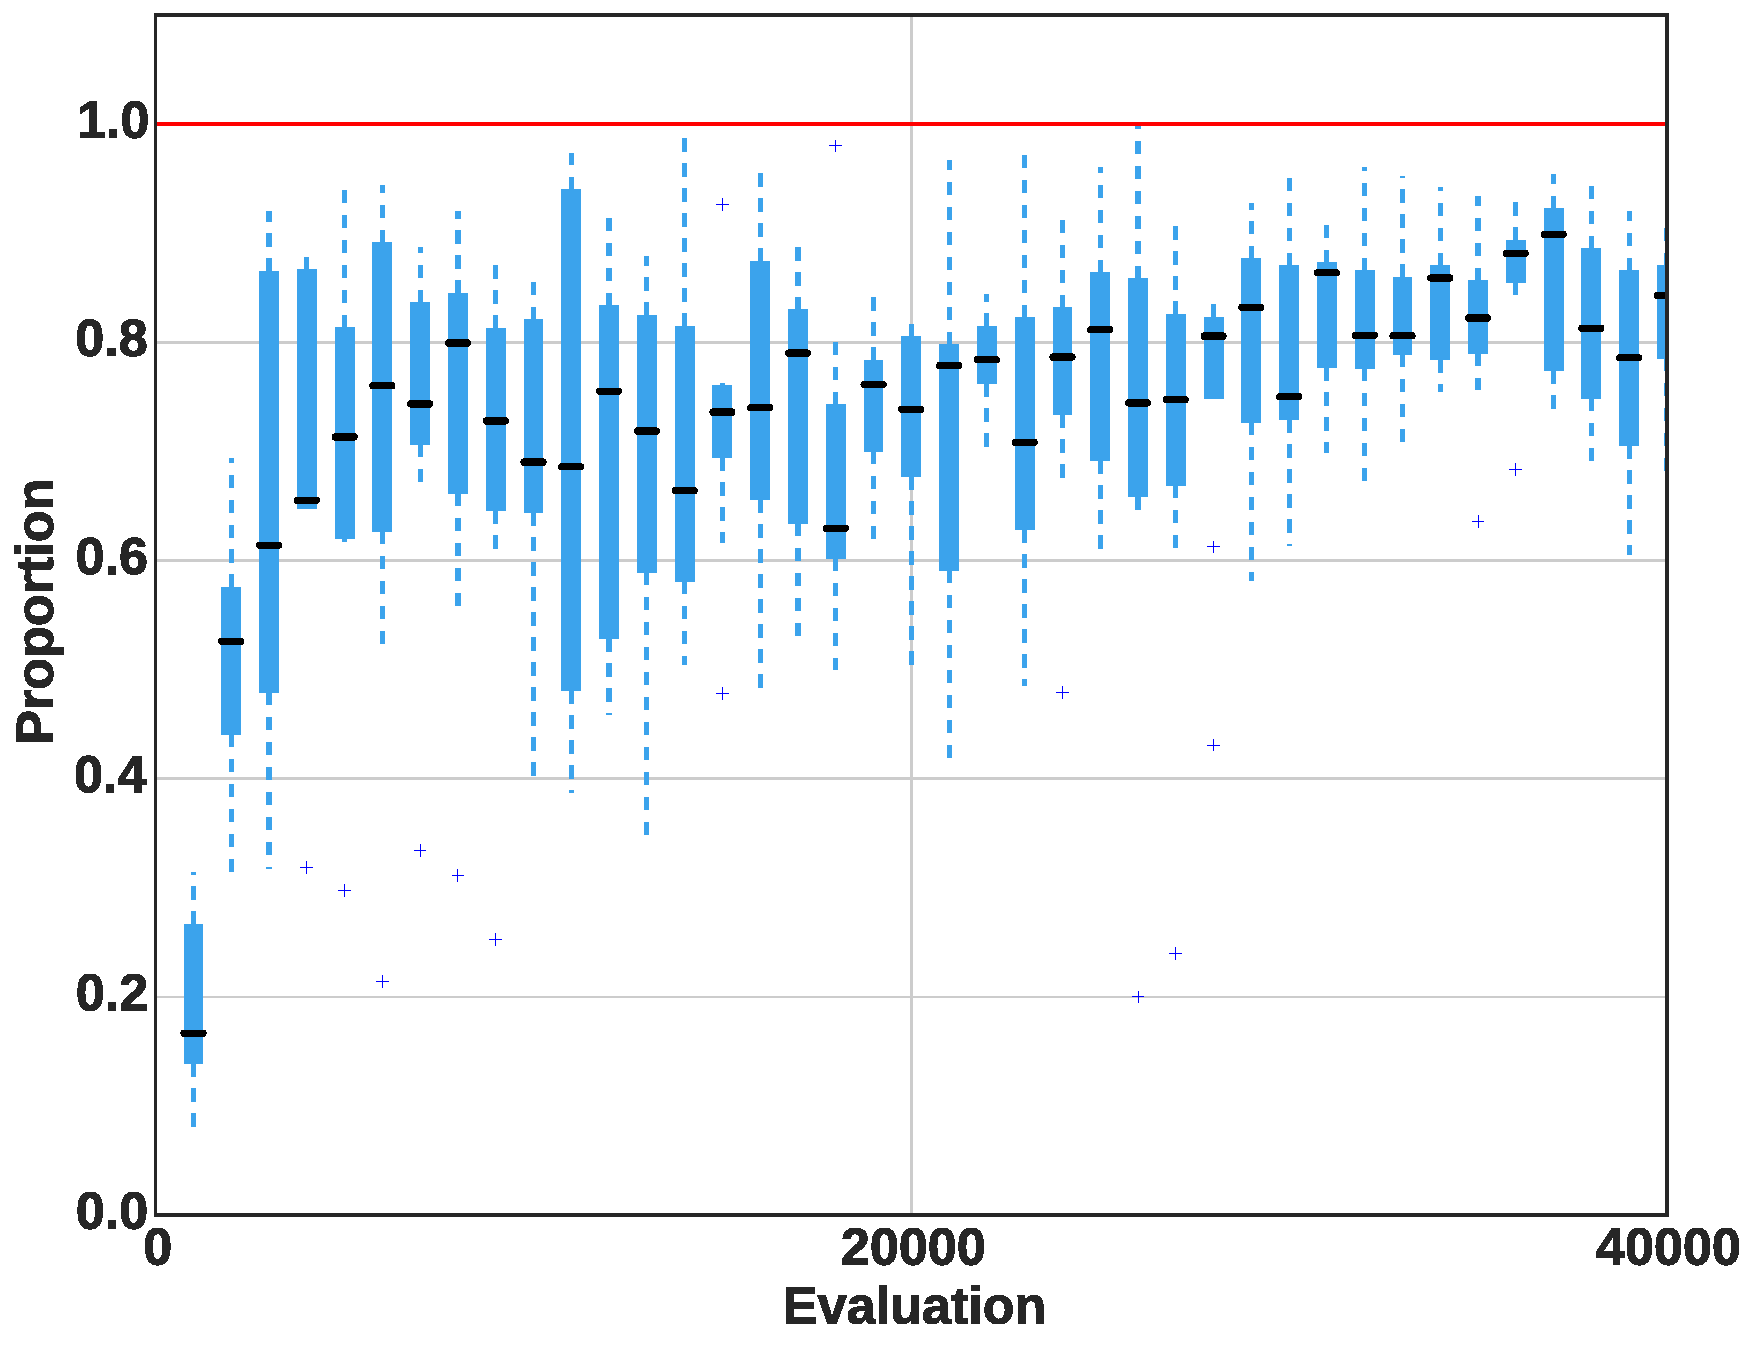
\includegraphics[scale=0.19]{fig/ArticleRob1/proportionLeadershipControl.pdf}}
      \end{subfigure}
      \begin{subfigure}[]
        {\label{fig:leadershipClonal} 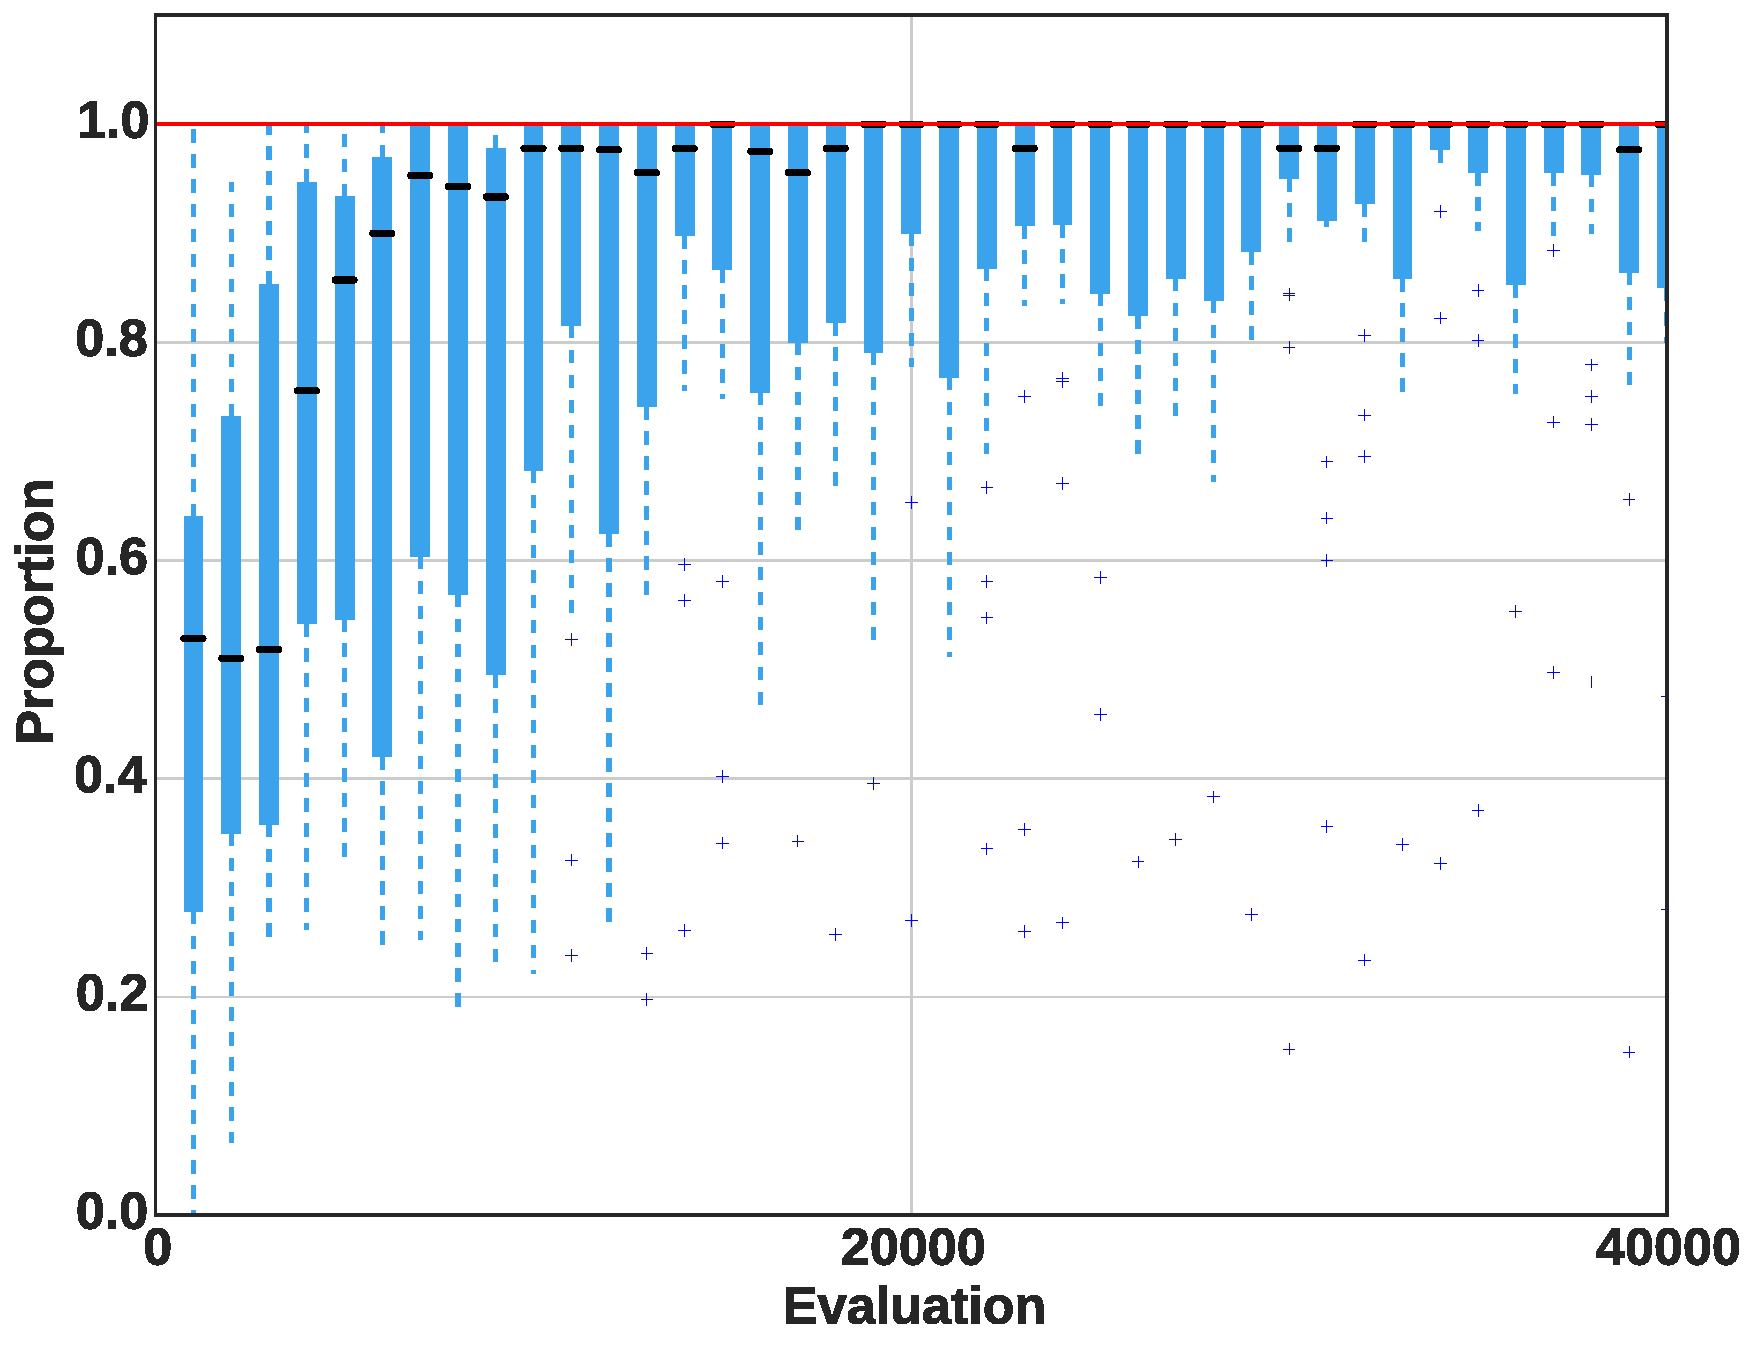
\includegraphics[scale=0.19]{fig/ArticleRob1/proportionLeadershipClonal.pdf}}
      \end{subfigure}
      \begin{subfigure}[]
        {\label{fig:leadershipCoevo} 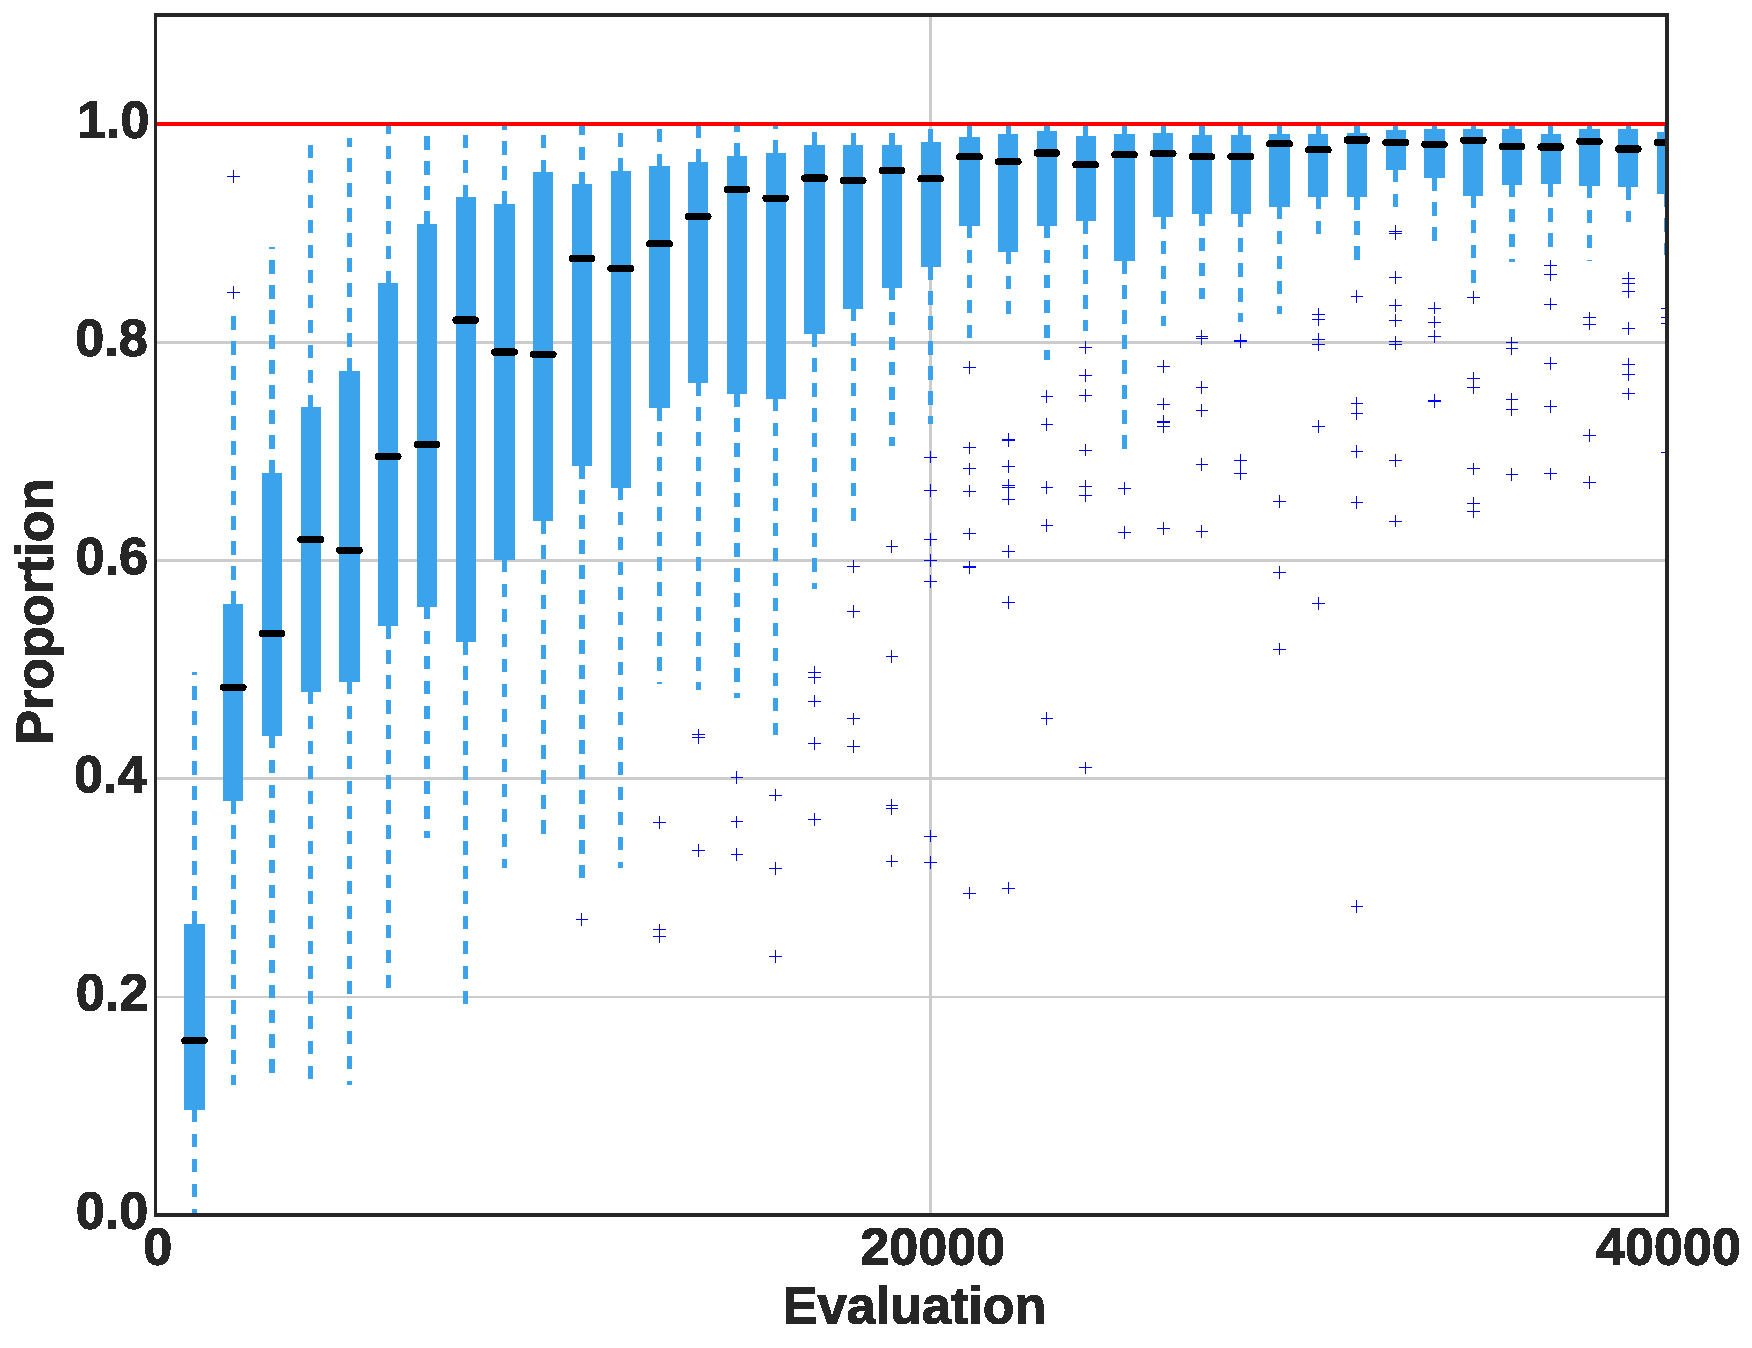
\includegraphics[scale=0.19]{fig/ArticleRob1/proportionLeadershipCoevo.pdf}}
      \end{subfigure}
      \caption{Boxplots of the proportion of leadership over time for the best individuals in each runs where the proportion at the last evaluation was greater than 0.75 in the {\em (a)}~control, {\em (b)}~clonal or {\em (c)}~coevolution setup. This value represents the proportion of waypoints crossed by both individuals for which the leader arrived first.}
      \label{fig:WaypointsLeadership}
  \end{figure}

  In the coevolution setup, nearly all runs (59/60) evolved a leader/follower strategy. Interestingly, although fitness scores in the clonal and control setups are significantly different, this behavior evolved in roughly one third of the runs for both setups. To explain the difference in fitness scores, we must take into account the quality of the leader/follower strategy in each setup. We measure the proportion of leadership in each interaction, which is computed as the proportion of waypoints crossed by both individuals for which the leader arrived first. Figure~\ref{fig:WaypointsLeadership} displays the boxplots of the proportion of leadership for the best individuals in each setup and only for the simulations where a successful leader/follower strategy evolved (a minimal threshold of 0.75 is chosen to consider only the best performing runs). We show that the proportion of leadership is greater in the clonal and coevolution setups than in the control one (Mann-Whitney, {\em p}-value $< 0.005$). These differences means that the individuals are more efficient in their leader/follower strategy in the clonal and coevolution settings than in the control one. This explains the differences in fitness scores observed in Figure~\ref{fig:WaypointsFitness}.

  Interestingly, whereas in the foraging task no leader/follower strategy could evolve in the control and clonal setups, this strategy did evolve in one third of the simulations for this task. This could mean that these individuals use information in the environment to adopt one role or the other. Indeed, we observe that this is achieved by exploiting the differences in the initial starting positions, with one individual on the left and the other on the right. They both turn to the same direction (left or right, depending on the runs) at the beginning of the simulation which results in one individual (the leader) turning its back to the other, while the second individual (the follower) looking at its partner. 


  \subsubsection{Recycling Cooperative Behaviors in the Foraging Task}

  Coming back to the initial foraging task, we perform the exact same experiment described at the beginning of this paper, with one notable exception: the initial population is initialized with genomes evolved for solving the waypoint task. This implies that coordination is possible starting from the very first generation of each setup. Given that we have already shown that such coordination is a desirable feature, the question is: will it be possible to retain cooperative behaviors in order to solve the foraging task?

  \begin{table}[hbtp]
    \center{
      \begin{tabular}{lcccc}
        \hline
        \multirow{2}{*}{\textbf{Setting}} & \multicolumn{2}{c}{\textbf{\# Coop.}} & \multirow{2}{*}{\textbf{\# Solitary}} & \multirow{2}{*}{\textbf{Total}}\\ 
        \cline{2-3}
         & \textbf{\# Lead.} & \textbf{\# Turn.} & & \\ 
        \hline
        \textit{Control} & 0 & 20 & 40 & \textbf{60}\\
        \textit{Clonal} & 0 & 24 & 36 & \textbf{60}\\
        \textit{Coevolution} & 28 & 0 & 32 & \textbf{60}\\
        \hline
      \end{tabular}
    }
    \caption{Proportion of the 60 independent simulations where the best individual evolved a cooperative strategy (collecting purple targets) or a solitary strategy (collecting green targets) for each setup in the foraging task when individuals are previously evolved in the waypoints task. In addition, the repartition of the different strategies is indicated when cooperation evolved: \emph{Leader/Follower} (Lead.) or \emph{Turning} (Turn.).}
    \label{tab:RecyclingCoopBehaviors}
  \end{table}

  Table~\ref{tab:RecyclingCoopBehaviors} gives the results in terms of evolved behaviors from the $60$ independent runs for each setup. 
  The coevolution setup evolves cooperation slightly more often (28/60) than both the control (20/60) and the clonal (24/60) setups. 
  A first remark is that the number of occurences of cooperation for the coevolution and control setups have actually doubled compared to previous results without incremental evolution (see Table~\ref{tab:ForagingCoop}). This is not the case for the clonal setup, which does not appear to benefit from incremental evolution. 

  A second remark is that cooperation in the coevolution setup systematically corresponds to a leader/follower strategy, which is \textit{never} the case with the two other setups. This has a significant, though expected, impact on fitness scores, as shown in Figure~\ref{fig:RecyclingFitness}. Cooperation evolved with the coevolution setup leads to significantly greater fitness scores (Mann-Whitney, {\em p}-value $<0.001$). 

  Results from this experiment make it possible to revise our initial statement. Using pre-trained individuals strongly benefits the coevolution setup in terms of evolvability. But this is not the case with the clonal setup, for which using pre-trained individuals improves neither evolvability nor efficiency. Therefore, we may face a tradeoff which does not concern evolvability and efficiency, but one that implies computational cost: the coevolution setup outperforms the clonal setup on both evolvability and efficiency \textit{at the cost of additional computational effort}.

  The control and clonal setups completely failed to maintain a leader/follower strategy, even though such strategy originally evolved. An explanation is provided by considering the difference between the waypoints task, where leader/follower evolved, and the current foraging task. In the waypoints task, symmetry breaking could be achieved at the beginning of the evaluation (as explained earlier), and could be retained afterwards as the follower was always behind the leader. However, the current foraging setup requires that the two robots display the same behavior to cooperatively collect a target (ie. both robots have to touch the target), which implies that leader/follower roles are lost, as they depend on the relative position of robots with one another. 


  \begin{figure}[hbtp]
    \begin{center}
      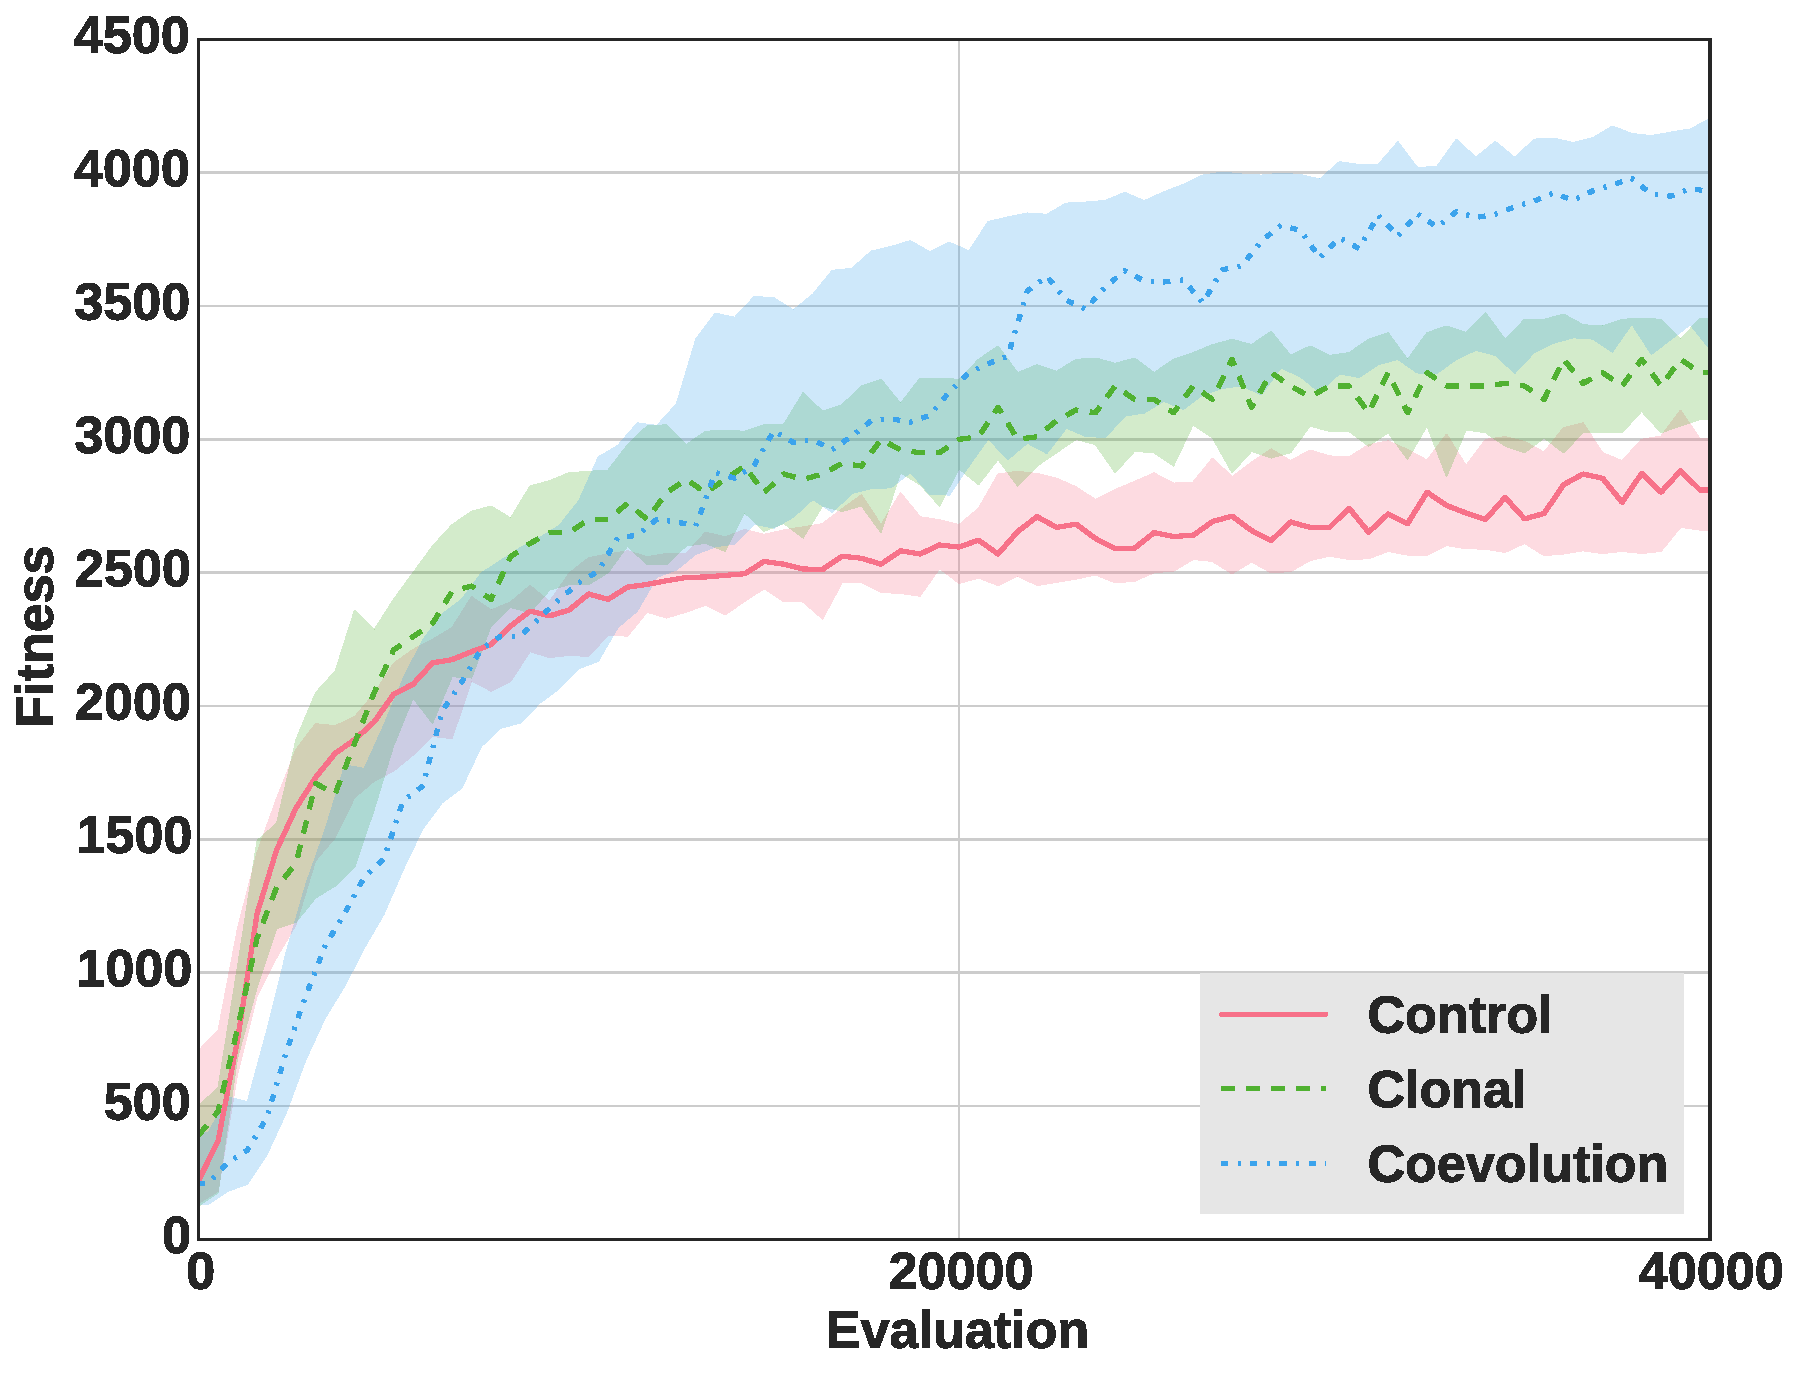
\includegraphics[scale = 0.3]{fig/ArticleRob1/fitnessRecyclingStags.pdf}
      \caption{Median fitness score of the best individuals in each of the runs where cooperation evolved for each setup over time. The fitness score of an individual is computed as the average reward the individual earned per trial by foraging targets. The colored areas around the medians represent the first and third quartiles.}
      \label{fig:RecyclingFitness}
      \end{center}
  \end{figure}

  \subsection{Discussion and Conclusion}

  In this paper, we considered several approaches for the evolution of cooperation in evolutionary robotics: a clonal approach, where all individuals in a group share the same genome, and a non-clonal approach, where individuals are independent from one another, but may share a common interest in cooperating. 

  We first showed that there exists a tradeoff between evolvability and efficiency. On the one hand, the clonal approach evolves cooperative behaviors on a more frequent basis than with the other approach. On the other hand, the non-clonal approach, which is implemented using a coevolution setup, results in more efficient behaviors in terms of pure performance whenever cooperation evolved. The non-clonal approach actually enables the evolution of asymmetric behaviors, such as a leader/follower strategy.

  We then used incremental evolution to evolve coordination behaviors using a simpler task in order to overcome this tradeoff and improve both evolvability and efficiency in each setup. We showed that while no improvement was observed in the clonal setup on either criteria, the outcome is very different for the coevolution setup: the probability of evolving cooperation actually increases, and the evolved cooperative solutions remain the most efficient.
 
  This work raises several questions. Firstly, heterogeneous behaviors were obtained with coevolution, a rather radical way to enable asymmetrical behaviors during cooperation. However, the waypoints task revealed that breaking symmetry can also be done with identical individuals using environmental feedback, even though such cooperation is difficult to obtain. As a consequence, we intend to investigate the evolution of cooperation with heterogeneous behavior without resorting to coevolution. In particular, we will study how more elaborated neural architectures (e.g. using plasticity) can switch to a particular persistant regime depending on environmental cues available at the beginning of the evaluation.

  Secondly, incremental evolution requires an added computational cost in order to increase evolvability in the non-clonal approach. However, it may be possible to avoid this extra cost by considering other evolutionary methods. In particular, we intend to explore how a multiobjective approach which considers both performance and \emph{diversity} could improve the optimization process~\cite{Lehman2008, Doncieux2014}. Though this approach looks promising, it is not clear yet how diversity should be implemented in the context of cooperative problem solving.


\section{Evolving Specialisation in a Population of Heterogeneous Robots: the Challenge of Bootstrapping and Maintaining Genotypic Polymorphism}
  \subsection{Introduction}
    Task specialisation is a defining characteristic in achieving efficient coordination and is thus considered to be crucial in the evolution of complex cooperative behaviours~\cite{Eors1995}. The problem of evolving cooperation has been largely studied in evolutionary robotics as it raises interesting persepectives for the design of collective robotics~\cite{Trianni2007, Hauert2014, Doncieux2015}. As a consequence, the manner in which robotic agents could evolve specialisation (or division of labour) for a cooperative task represents a compelling challenge in evolutionary robotics. As such, a large body of litterature has already been dedicated to this subject. However, most research focus on the particular case of homogeneous groups of individuals~\cite{Waibel2009} as is classic in evolutionary robotics. This means that the individuals are forced to rely on phenotypical plasticity~\cite{Waibel2006, Ferrante2015, Eskridge2015} and/or environmental cues~\cite{Waibel2006, Goldsby2010} in order to achieve specialisation. In comparison, the evolution of specialisation in a population of unrelated individuals has been mostly ignored.

    Yet achieving division of labour under such conditions raises an interesting problem: because individuals cannot dynamically specialise during evaluation, the division needs to occur at the genotypic level. Thus it poses the problem of both \emph{evolving} and \emph{maintaining} genotypic polymorphism in a single population. Here we investigate the conditions under which specialised behaviours for a cooperative task can evolve in a single population of heterogeneous individuals. In particular, we are interested in the influence of the selection process in achieving division of labour. 

    We design a 2-robots cooperative foraging task where both a solitary and a cooperative strategies can evolve but where cooperation is highly rewarded. The genotype of each robotic agent is separately chosen in the population and the individuals therefore form an heterogeneous group. This task is greatly favored by the evolution of efficient coordination strategies. In particular, our previous work on a similar task~\cite{Bernard2015} showed that two types of cooperative strategy could evolve: one where both individuals adopt homogeneous behaviours (generalists) and the other one where they adopt a leader/follower strategy (specialists). As the latter is the more efficient one we study the conditions for its emergence. The evolutionary dynamics of two popular selection methods are studied: (1) an elitist \((\mu + \lambda)\) selection scheme and (2) a fitness-proportionate selection scheme. Fitness-proportionate in particular is interesting with regards to genotypic polymorphism as it is known to allow the evolution of frequency-dependent selection~\cite{Altenberg1991}.

    In the next Section, we introduce the experimental setup. Then we present the two types of successful cooperative strategies that may evolve. Next, we investigate whether any of the selection methods could evolve heterogeneous behaviours. In particular, we study for both schemes the evolutionary outcomes depending on whether the population is initially constituted of random individuals or seeded with pre-evolved efficient specialists. Then we present the results of computational analyses in order to reveal and understand more deeply the mechanisms at play. In a final experiment, we reveal two key properties required for the evolution of heterogeneous behaviours, and discuss the implications of our work.




  \subsection{Methods}
  \label{sec:methods}
    We evaluate two robotic agents in a $800$ by $800$ units square arena devoid of any obstacle except for the foraging targets. At the beginning of a simulation, $18$ targets are randomly positioned in the environment. While the agents may move freely in the arena, the targets' positions are fixed. For a target to be collected, any agent needs to stay in contact with it for a specified amount of time ($800$ simulation steps). The target is removed after this duration and put back at another random position so that the number of targets is kept the same throughout a simulation. We consider that cooperative foraging happens if both individuals are in contact of the target when it is removed. When an agent collects a target, it is rewarded 50 if this target has been foraged in a solitary manner or 250 if both agents have cooperated to collect it.

    Each agent is circular-shaped with a diameter of $20$ units and possesses a collection of different sensory inputs. The first type of inputs is a $90$ degrees front camera and is composed of $12$ rays, each one indicating the type and distance to the nearest object (either another agent or a target). The other type of inputs are $12$ proximity sensors evenly distributed around the agent's body. With a range of twice the agent's diameter, each proximity sensor outputs the proximity of the nearest obstacle in its range.

    Both agents begin the simulation next to each other at the same end of the arena and can move according to the outputs of their neural network. This neural network is a fully connected multi-layer perceptron with one hidden layer. The inputs of the neural network are comprised of all the sensory information of the agent, i.e. $36$ input neurons for the camera ($3$ inputs for each ray) and $12$ for the proximity sensors. A final input neuron whose value is always $1$ is used as a bias neuron. This amounts the total number of input neurons to $49$. The hidden layer is constituted of $8$ neurons while the $2$ neurons of the output layer return the speed of the agent's wheels. A sigmoid is used as the activation function of each neuron. Finally, the topology of the network is kept constant during the experiments.

    The population of individuals is evolved thanks to a classical evolutionary algorithm. The genotype of each individual is constituted of a collection of the $410$ real-valued connection weights of the neural network. At each generation of the algorithm, every individual is evaluated by being paired $5$ times with other individuals randomly chosen in the population (i.e. $5$ 1-to-1 pairing). Each pair interacts in the setting presented before during $20000$ simulation steps which we call a \emph{trial}. We perform $5$ trials for each pair of individuals in order to decrease the impact of the targets' random positions on the individuals' performance. The fitness score (\(F\)) of an individual is computed as the average reward per trial:

    \[
    F = \frac{1}{N*M} \sum_{i=1}^{N} \sum_{j=1}^{M} f_{ij}
    \]

    with \(N\) the number of partners the individual is paired with ($5$), \(M\) the number of trials with each partner ($5$) and \(f_{ij}\) the sum of rewards obtained at trial \(j\) with partner \(i\).

    The population for the next generation is created according to two different selection schemes:

    \begin{itemize}
      \item{\textbf{\((\mu + \lambda)\) elitist selection:} the population of the next generation is constituted of the $\mu$ best individuals from this generation and $\lambda$ offsprings built from the best individuals.}
      \item{\textbf{Fitness-proportionate:} offsprings are built by sampling individuals from the current generation to constitute the population of the next generation. The probability to sample a particular parent is proportional to this parent's fitness score.}
    \end{itemize}

    Regardless of the selection method used, every offspring is a mutated clone of its parent and no recombination is used in our algorithm. The probability for each gene to mutate is \(5 \times 10^{-3}\) and mutations are sampled according to a gaussian operator with a standard deviation of \(2 \times 10^{-2}\). Finally, experiments were conducted with the robotic 2D simulator of SFERESv2~\cite{Mouret2010}, a framework for evolutionary computation. Source code for the experiments is available for download at http://pages.isir.upmc.fr/\textasciitilde bredeche/Experiments/ALIFE2016-specialisation.tgz
    

  \subsection{Behaviours of Specialists in a Cooperative Foraging Task}
  \label{sec:efficiency}
    We showed in a previous article~\cite{Bernard2015} that two cooperative strategies could evolve in this particular task: \emph{turning} (between two \emph{turners}) and \emph{leader/follower} (between a \emph{leader} and a \emph{follower}). Both of these strategies achieve cooperative foraging but with varied efficiency.

    \begin{figure}[hbtp]
      \centering
        \begin{subfigure}[]
          {\label{fig:behaviorTurning} 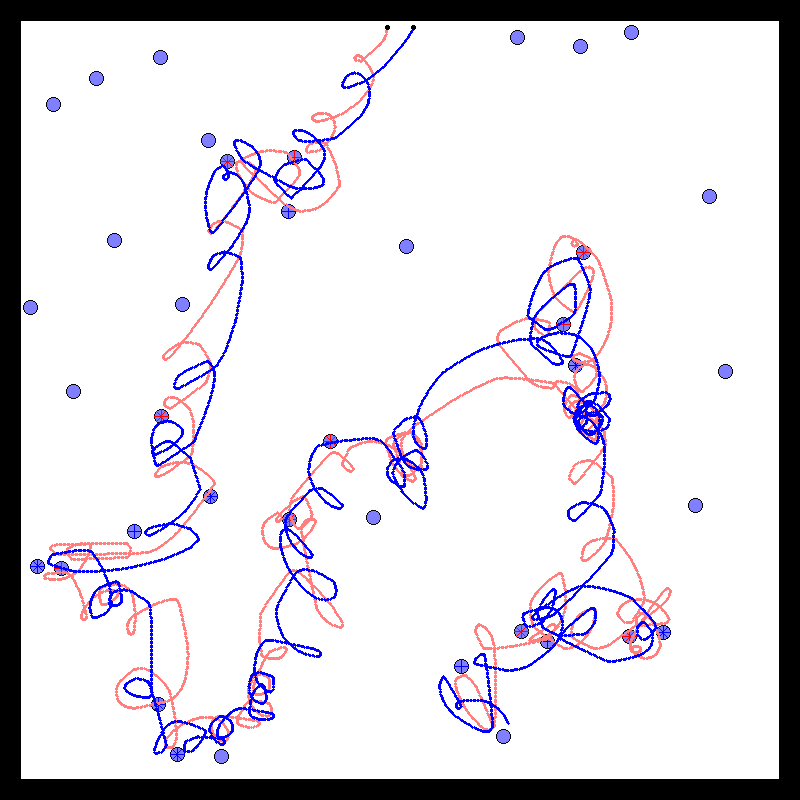
\includegraphics[scale=0.14]{fig/ArticleRob2/behaviorTurning.png}}
        \end{subfigure}~
        \begin{subfigure}[]
          {\label{fig:behaviorLeadership} 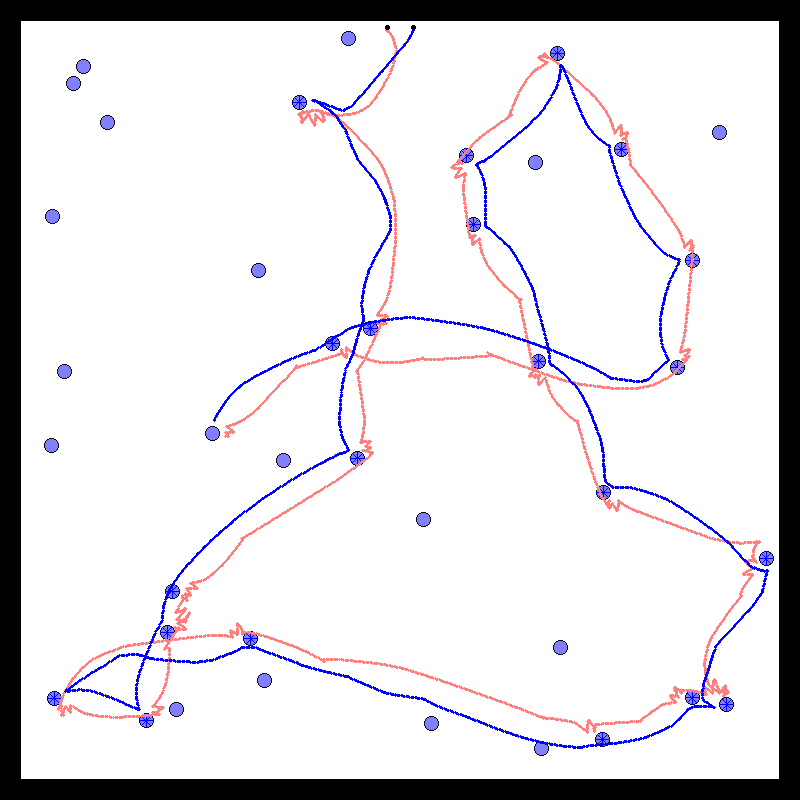
\includegraphics[scale=0.14]{fig/ArticleRob2/behaviorLeadership.png}}
        \end{subfigure}
        \caption{\textbf{Snapshots of the simulation after an entire trial in the foraging task.} The path of each robotic agent from their initial positions (black dots) is represented in red and blue. The blue discs represent the 18 targets in the environment. When a target is foraged by the two agents, a red cross (resp. blue) is drawn on the target if the red agent (resp. blue) arrived on it first. Each snapshot corresponds to a trial where agents adopted a different behavior: {\em (a)}~turning or {\em (b)}~leader/follower.}
        \label{fig:behaviorTraces}
    \end{figure}

    In the turning strategy, both individuals turn around one another so that they can keep the other individual in their line of sight and stay close to it (see Figure \ref{fig:behaviorTurning}). At the same time, the two individuals try to get closer to a target. This way, as soon as one of the two individuals is in contact with a target, the other individual can join it so the target may be collected cooperatively. Consequently, both individuals adopt a similar behaviour in this strategy and can be described as generalists.

    In the leader/follower strategy, the individuals specialise in two roles: a \emph{leader} and a \emph{follower}. The \emph{leader} always gets on the target first and checks rarely for its partner. In comparison, the \emph{follower} tries to keep its \emph{leader} in view during the entirety of the simulation so that it can get on the same target (see Figure \ref{fig:behaviorLeadership}). Consequently, we observe the expression of two clearly heterogeneous behaviours which implies that both individuals are specialists.

    \begin{figure}[hbtp]
      \centering
        \begin{subfigure}[]
          {\label{fig:Efficiency} 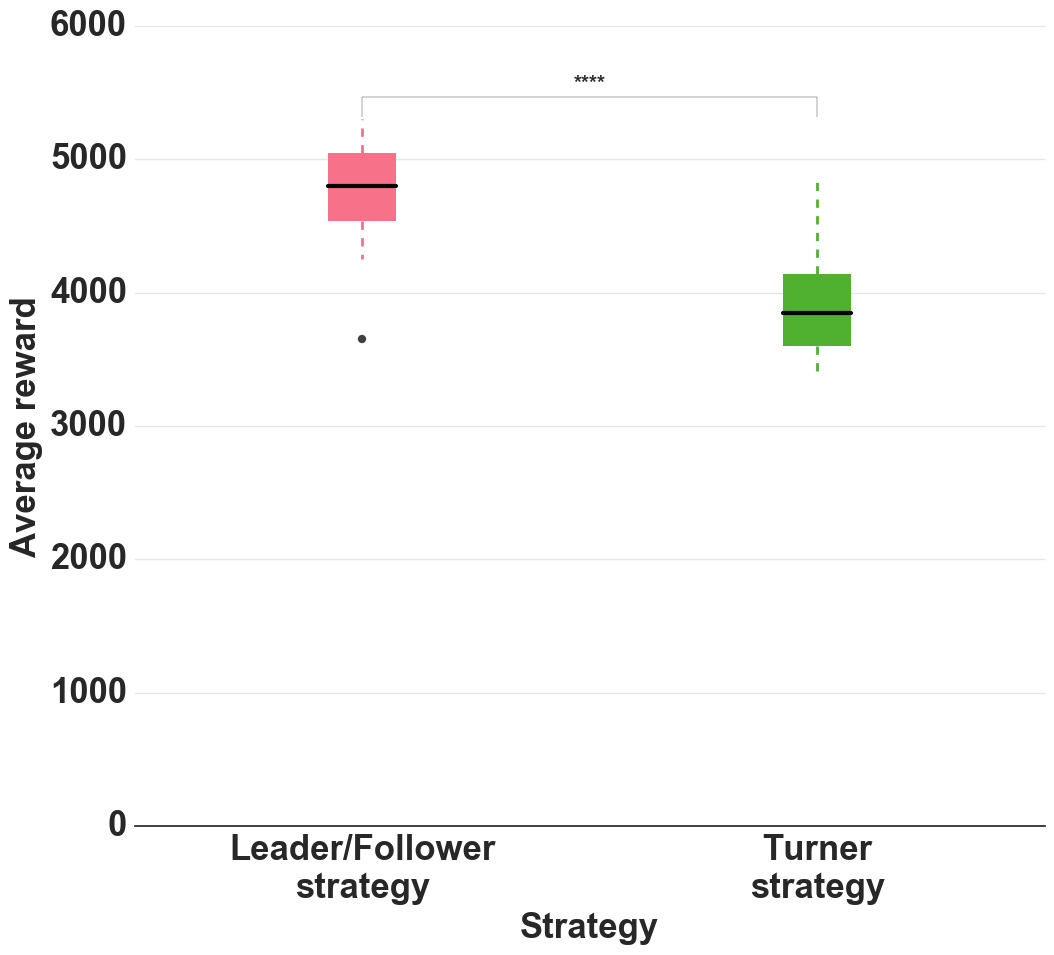
\includegraphics[scale=0.25]{fig/ArticleRob2/boxplotFitness.png}}
        \end{subfigure}~
        \begin{subfigure}[]
          {\label{fig:Leadership} 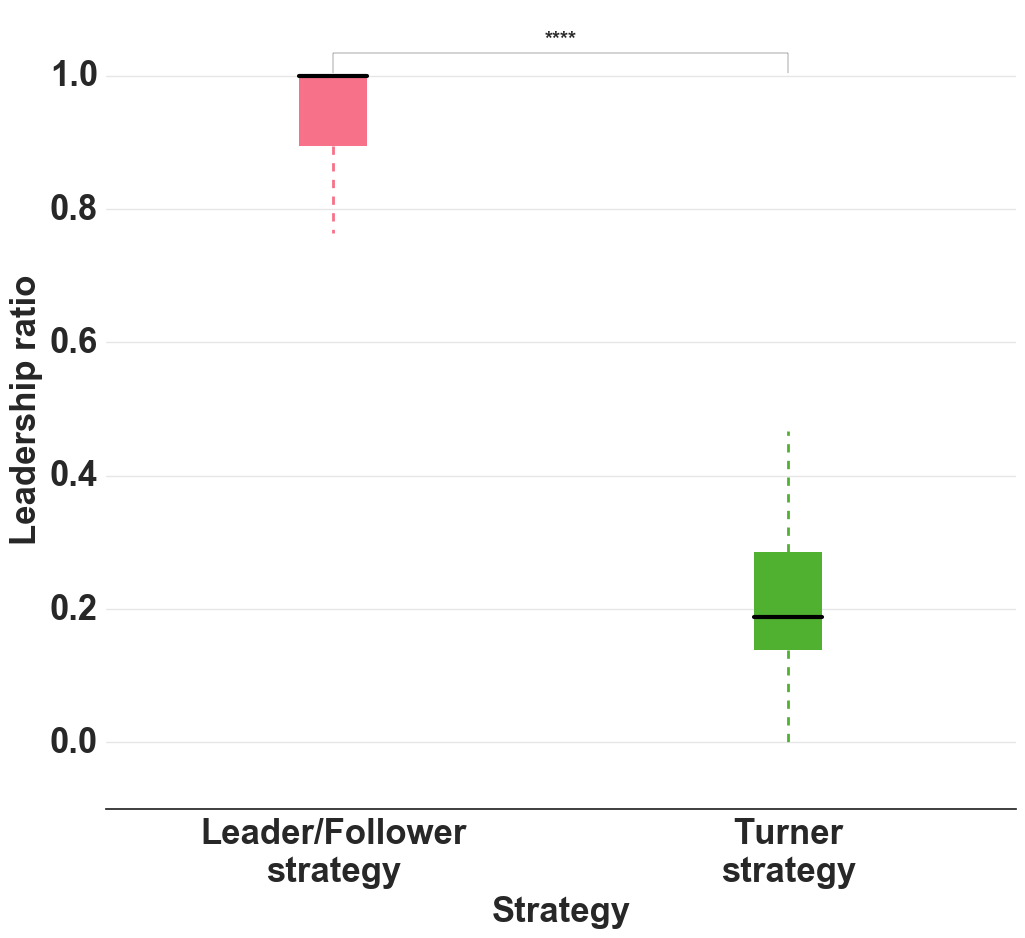
\includegraphics[scale=0.25]{fig/ArticleRob2/boxplotLeadership.png}}
        \end{subfigure}
        \caption{\textbf{Average reward and leadership proportion with a leader/follower or turning strategy} Boxplots of {\em (a)}~the average reward and {\em (b)}~the leadership proportion over $20$ independent trials for the leader/follower and turning strategies. The leadership ratio of an individual represents the propensity for one individual among the pair to arrive first more often than its partner on a target collected in a cooperative fashion. The position of each target at the beginning of each trial was randomized.}
        \label{fig:EfficiencyAndLeadership}
    \end{figure}

    Figure~\ref{fig:Efficiency} shows the efficiency of each strategy, defined as the average reward obtained of the two individuals during a simulation over $20$ independent trials (with randomized targets' positions for each trial). We can see that, as expected, the leader/follower strategy achieves a significantly higher efficiency (Mann-Whitney U-test on the average reward over $20$ trials, {\em p}-value $< 0.0001$). This difference in efficiency is directly correlated to a highly significant difference in the proportion of leadership as shown in Figure~\ref{fig:Leadership} (Mann-Whitney U-test on the leadership proportion over $20$ trials, {\em p}-value $< 0.0001$). We compute this proportion by looking at the propensity for one of the two individuals to arrive first more often on a target foraged cooperatively.



  \subsection{Evolving Heterogeneous Behaviours with an Elitist Selection}
  \label{sec:elitistEvolution}
    \subsubsection{Bootstrapping leader/follower strategies}
      In this first experiment, we are interested in the emergence of a leader/follower strategy when starting with a population of random individuals under an \((\mu + \lambda)\) elitist selection. In order to investigate the influence of population size, we tested three different sizes \(N\): $20$, $40$ and $100$. For each population size, we conducted $11$ independent runs, each one lasting $90000$ evaluations. For each population size \(N\), we defined \(\mu\) (i.e. the number of parents) and \(\lambda\) (i.e. the number of offsprings) as follows:
        \[
          \mu = \frac{N}{2}, 
          \lambda = \frac{N}{2}
        \]

      For example, when population size was $100$, $50$ individuals were kept from the previous generation and used to create $50$ mutated offsprings.

      \begin{table}[hbtp]
        \center{
          \begin{tabular}{lcccc}
            \hline
            \textbf{Pop.} & \textbf{\# L/F} & \textbf{\# Turning} & \textbf{\# NC} & \textbf{Total}\\ 
            \textbf{size} & \textbf{Strat.} & \textbf{Strat.} & \textbf{Strat.} & \\ 
            \hline
            \textit{20} & 0 & 11 & 0 & \textbf{11}\\
            \textit{40} & 0 & 11 & 0 & \textbf{11}\\
            \textit{100} & 1 & 10 & 0 & \textbf{11}\\
            \hline
          \end{tabular}
        }
        \caption{\textbf{Strategies evolved by the best individuals under elitist selection with an initially random population.} Repartition of the different strategies adopted by the best individuals at the last evaluation in each of the replicates for different population sizes \(N\). We indicate in each cell the number of simulations where a particular strategy evolved. Populations were evolved under an \((\mu + \lambda)\) elitist selection, with \(\mu = \frac{N}{2}\) and \(\lambda = \frac{N}{2}\). Individuals' genotype values were intially random. In the table "L/F" stands for leader/follower and "NC" for "Non-Cooperative".}
        \label{tab:elitistScratchStrategies}
      \end{table}

      Table~\ref{tab:elitistScratchStrategies} shows the repartition of the best individuals' strategies at the last generation of evolution for each population size. We consider a behaviour to be cooperative when more than 50\% of the total number of targets collected are foraged cooperatively. First we observe that in every replicates, individuals always end up evolving a cooperative strategy. We also see that evolving a leader/follower strategy is difficult as specialists evolve in only $1$ run (out of $33$) and when the population size is $100$. These results suggest that it is nearly impossible to evolve such heterogeneous behaviours with this setting.

      However, when looking at the whole evolutionary history we can reveal additional information about the evolution of specialists. We show in Figure~\ref{fig:leadershipTime} the proportion of evolutionary time when the best individual of each run adopted a leader/follower strategy. This value is computed as the ratio of the number of generations when the leadership ratio was high enough (threshold value of $0.6$) out of the total number of generations. We observe that even if the best individuals end up adopting a generalist strategy, this was not the case during the entirety of the evolution. In particular, there is a significant increase (Mann-Whitney, {\em p}-value $< 0.05$) in the number of generations where the best individual showed a leader/follower strategy when population size was $100$ compared to a population size of $20$. Therefore this implies that it is possible to evolve specialists but their stability in the population over time is nearly impossible to achieve.

      \begin{figure}[hbtp]
        \centering
          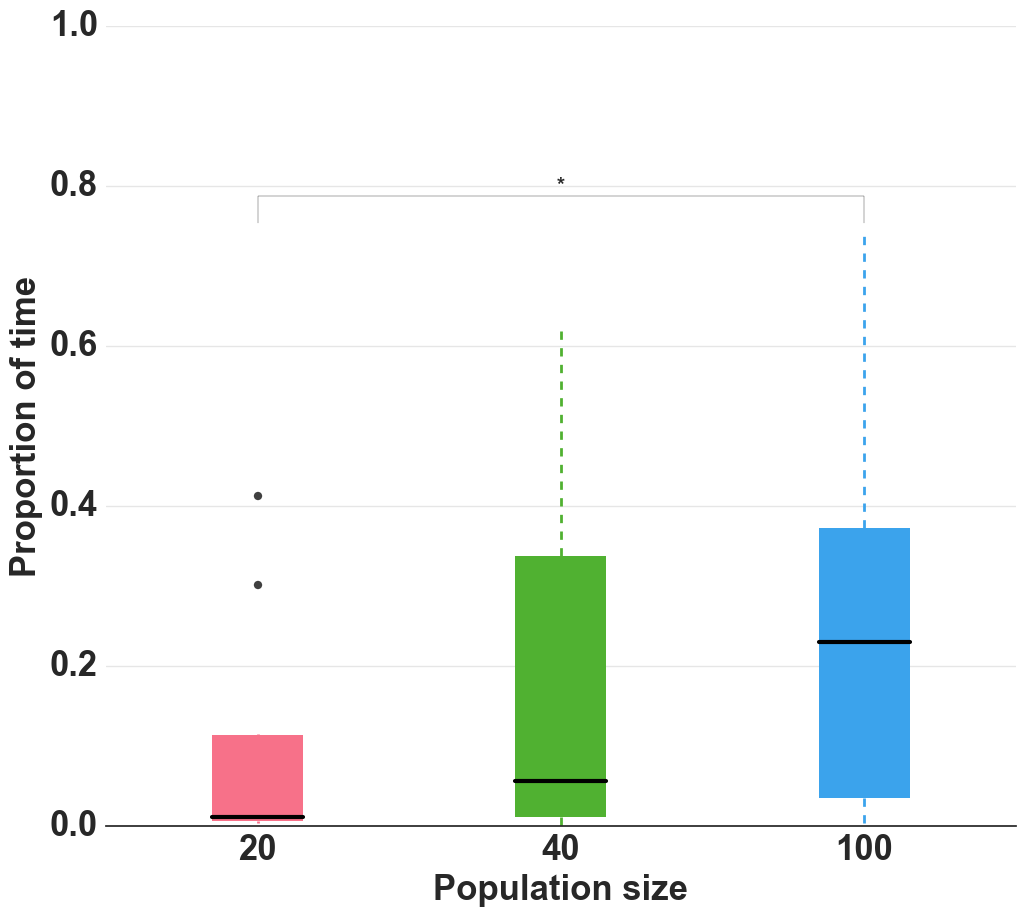
\includegraphics[scale=0.25]{fig/ArticleRob2/boxplotLeadershipTime.png}
          \caption{\textbf{Proportion of time with a leader/follower strategy.} Boxplots of the number of generations when the best individual in each replicate adopted a leader/follower strategy out of the total number of generations. We consider that the best individual adopted a leader/follower strategy when its leadership ratio was over a threshold value of $0.6$.}
        \label{fig:leadershipTime}
      \end{figure}


    \subsubsection{Maintaining heterogeneity in a population seeded with specialists}
      In order to investigate the lack of stability of genotypic polymorphism under elitist selection, we design another experiment. We separately evolve a population of non-cooperators, which we call \emph{solo} individuals (i.e. \emph{leaders}), and efficient \emph{follower} beforehand. We then replace the worst individuals w.r.t. fitness score in the population of solo individuals by a certain amount of \emph{followers}. Our goal is to study if artificially constructing such population could result in the invasion and fixation of a stable leader/follower strategy.

      The number of \emph{followers} initially inserted in the population was varied according to two different settings: (1) we add only one \emph{follower} or (2) we add an amount of \emph{followers} equal to half of the population. Experiments were replicated $11$ times during $90000$ evaluations with population size of $40$ and $100$.

      \begin{table}[hbtp]
        \center{
          \begin{tabular}{lrcccc}
            \hline
            \textbf{Pop.} & \textbf{Followers} & \textbf{\# L/F} & \textbf{\# Turning} & \textbf{\# NC} & \textbf{Total}\\ 
            \textbf{size} & \textbf{added} & \textbf{Strat.} & \textbf{Strat.} & \textbf{Strat.} & \\ 
            \hline
            \textit{40} & \textit{1} & 0 & 11 & 0 & \textbf{11}\\
            \textit{40} & \textit{20} & 0 & 11 & 0 & \textbf{11}\\
            \textit{100} & \textit{1} & 1 & 10 & 0 & \textbf{11}\\
            \textit{100} & \textit{50} & 2 & 9 & 0 & \textbf{11}\\
            \hline
          \end{tabular}
        }
        \caption{\textbf{Strategies evolved by the best individuals with elitist selection when adding \emph{followers}.} Repartition of the different strategies adopted by the best individuals at last evaluation in each of the replicates for different population sizes \(N\). We indicate in each cell the number of simulations where a particular strategy evolved. Populations were evolved under a \((\mu + \lambda)\) elitist selection, with \(\mu = \frac{N}{2}\) and \(\lambda = \frac{N}{2}\). The population was initially seeded with a population of \emph{solo} individuals in which we added a specific amount of \emph{followers}. In the table "L/F" stands for leader/follower and "NC" for "Non-Cooperative".}
        \label{tab:elitistInvasionStrategies}
      \end{table}


      We show (Table~\ref{tab:elitistInvasionStrategies}) no significant differences in comparison with a population constituted of initially random individuals w.r.t. the number of simulations where a leader/follower strategy evolved. These results suggest that even when purposely adding specialists, their stability in the population is still very hard to achieve. This implies that whether the behaviours are evolved from random genotypes or bootstrapped with efficient individuals is not as important as maintaining heterogeneity in the population. In particular, in only one replicate among the $3$ runs where a leader/strategy was eventually adopted (out of $44$) did the specialists initially added were maintained. In the $2$ other runs we observe multiple emergences and disappearances of specialists throughout evolution. 

      % TODO: Mentionner que néanmoins le leader/follower est globalement plus stable comparé du from scratch ?
      % However, it is interesting to note that the addition of efficient followers lead to more stable heterogeneity than when starting from scratch [TODO: GRAPH LEADERSHIP TIME].


  \subsection{Evolution Under a Fitness-Proportionate Selection}
  \label{sec:fitpropEvolution}
    In this next experiment we want to investigate the evolution of heterogeneous behaviours when using a fitness-proportionate selection. As fitness-proportionate is known to allow frequency-dependent selection, we hypothesize that it may facilitate the evolution of specialists.

    \subsubsection{Bootstrapping leader/follower strategies}
      Similarly to the elitist selection, we replicated our experiments in $11$ independent runs during $90000$ evaluations. Likewise, population sizes were $20$, $40$ and $100$. 
      
      \begin{table}[hbtp]
        \center{
          \begin{tabular}{lcccc}
            \hline
            \textbf{Pop.} & \textbf{\# L/F} & \textbf{\# Turning} & \textbf{\# NC} & \textbf{Total}\\ 
            \textbf{size} & \textbf{Strat.} & \textbf{Strat.} & \textbf{Strat.} & \\ 
            \hline
            \textit{20} & 0 & 1 & 10 & \textbf{11}\\
            \textit{40} & 0 & 1 & 10 & \textbf{11}\\
            \textit{100} & 1 & 2 & 8 & \textbf{11}\\
            \hline
          \end{tabular}
        }
        \caption{\textbf{Strategies evolved by the best individuals under fitness-proportionate selection with an initially random population.} Repartition of the different strategies adopted by the best individuals at the last evaluation in each of the replicates for different population sizes. We indicate in each cell the number of simulations where a particular strategy evolved. Populations were evolved under a fitness-proportionate selection. Individuals' genotype values were initially random. In the table "L/F" stands for leader/follower and "NC" for "Non-Cooperative".}
        \label{tab:fitpropScratchStrategies}
      \end{table}

      We show in Table~\ref{tab:fitpropScratchStrategies} that results are highly different when using such selection scheme. In particular, the fitness-proportionate selection performed poorly w.r.t. evolving cooperative strategies. For each population size, no cooperative strategy evolved at all in the vast majority of replicates. However in one particular run we do observe the emergence and fixation of specialists. This would suggest that fitness-proportionate may perform equally as an elitist selection w.r.t. the evolution of heterogeneous behaviours. 

      Yet a closer look at the dynamics of evolution under a fitness-proportionate selection yields interesting results. In particular, there is not much variation in the strategy adopted by the best individuals throughout evolution. This is consistent with the fact that the bootstrap of a cooperative strategy was not observed in most of the replicates: fitness-proportionate is not efficient in evolving any cooperative behaviour. In consequence, there is not much variation in the proportion of individuals adopting a leader/follower strategy during evolution. As a matter of fact, we observe that in the only replicate where there was genotypic polymorphism at the end of the simulation, specialists were already present at the random initialisation of the population and did not evolve through mutation. This is very different with the elitist selection where we observe multiple emergences of specialists (even briefly) during evolution in many different runs.

    \subsubsection{Maintaining heterogeneity in a population seeded with specialists}
      \begin{table}[hbtp]
        \center{
          \begin{tabular}{lrcccc}
            \hline
            \textbf{Pop.} & \textbf{Followers} & \textbf{\# L/F} & \textbf{\# Turning} & \textbf{\# NC} & \textbf{Total}\\ 
            \textbf{size} & \textbf{added} & \textbf{Strat.} & \textbf{Strat.} & \textbf{Strat.} & \\ 
            \hline
            \textit{40} & \textit{1} & 7 & 0 & 4 & \textbf{11}\\
            \textit{40} & \textit{20} & 8 & 0 & 3 & \textbf{11}\\
            \textit{100} & \textit{1} & 10 & 0 & 1 & \textbf{11}\\
            \textit{100} & \textit{50} & 10 & 0 & 1 & \textbf{11}\\
            \hline
          \end{tabular}
        }
        \caption{\textbf{Strategies evolved by the best individuals with fitness-proportionate selection when adding \emph{followers}.} Repartition of the different strategies adopted by the best individuals at the last evaluation in each of the replicates for different population sizes \(N\). We indicate in each cell the number of simulations where a particular strategy evolved. Populations were evolved under a fitness-proportionate selection. The population was initially seeded with a population of \emph{solo} individuals in which we added a specific amount of \emph{followers}. In the table "L/F" stands for leader/follower and "NC" for "Non-Cooperative".}
        \label{tab:fitpropInvasionStrategies}
      \end{table}

      As expected from previous results, fitness-proportionate performs well in terms of stability of heterogeneous behaviours. We show in Table~\ref{tab:fitpropInvasionStrategies} that in the majority of replicates the best individuals adopt a leader/follower strategy at the end of the simulations. This is particularly true when population size is high enough ($100$). A major difference with the elitist selection is that in all replicates where a leader/follower strategy was observed at the end of the run, the specialists were maintained from the start throughout evolutionary time. These results suggest that, although not efficient at bootstrapping cooperative behaviours, fitness-proportionate performs well w.r.t. the stability of genotypic heterogeneity.


    \subsection{Computational Analyses of Population Dynamics}
      In this Section, we aim at understanding more deeply the dynamics at play that allow the invasion of suboptimal generalists even when efficient specialists are present. To that end we run computational analyses based on the expected fitness of each of the three phenotypes. Table~\ref{tab:payoffMatrix} shows the average payoff of pair-wise simulations between each type of phenotypes. We consider the payoffs for both phenotypes in each pair to be identical as no significant differences were observed between their payoffs.

      \begin{table}[hbtp]
        \center{
          \begin{tabular}{cccc}
            \hline
            \textbf{Phenotype} & \textit{Solo} & \textit{Follower} & \textit{Turner} \\
            \hline
            \textit{Solo} & 1265 & 5000 & 3480 \\
            \textit{Follower} & 5000 & 100 & 2750 \\
            \textit{Turner} & 3480 & 2750 & 2755 \\
            \hline
          \end{tabular}
        }
        \caption{\textbf{Payoff matrix for pair-wise simulations of each phenotype.} Average payoffs of each phenotype against every phenotype in a pair-wise simulation. Each pair was evaluated $10$ times in order to decrease the stochastic effects of the initial conditions (i.e. random positions of the targets).}
        \label{tab:payoffMatrix}
      \end{table}

      Several observations can be made directly from these results. First, we can confirm that the leader/follower strategy displayed by a (\emph{solo}, \emph{follower}) pair is clearly the best strategy. However each one of these two phenotypes performs very poorly against itself with the worst payoff obtained by a pair constituted of two \emph{followers}. Secondly, \emph{turner} individuals perform also very well against \emph{solo} individuals. Last, there is no significant differences w.r.t. payoffs when a \emph{turner} is paired with a \emph{follower} or another \emph{turner}. These last two points hint at a shared lineage between \emph{followers} and \emph{turners}. 

      Indeed analyses of the genotypes' histories in our previous experiments reveal that \emph{turner} individuals in fact descend from \emph{follower} individuals. This means that they act as \emph{followers} when interacting with \emph{solo} individuals but are not as efficient. However they are a lot more efficient than \emph{followers} when paired with individuals of the same phenotype (or \emph{followers}).

      % TODO: Virer le paragraphe précédent ? (notamment pour faire un peu de place)

      From this payoff matrix, we run computational analyses to model the gradient of phenotypes' repartition in an infinite population. The fitness \(W\) of a particular phenotype \(i\) is computed as follows:

      \[
        W_{i} = \sum_{j=1}^{M} P(ij)*F(j)
      \]

      with \(j\) the phenotype it is paired with, \(M\) the number of different phenotypes ($3$), \(P(ij)\) the payoff of phenotype \(i\) against \(j\) and \(F(j)\) the proportion of phenotype \(j\) in the population. From this fitness, we can deduce the variation of phenotypes repartition by updating the proportion \(F\) of each phenotype \(i\): 

      \[
        F_{i} = F_{i}*\frac{W_{i}}{\sum_{j=1}^{M} W_{j}}
      \]

      We show in Figure~\ref{fig:expectations} a vector field of this gradient. We can see that there actually exists an equilibrium between the three phenotypes (marked by a black dot at the crossing between the dashed lines). This implies that even though the \emph{turner} strategy is the not the more efficient one, it is still expected that this phenotype can invade and coexists with the other two phenotypes.

      We can hypothesize that we could not observe this equilibrium in our robotic simulations because of the stochastic effects arising from selection in a finite population. In order to study this hypothesis we ran additional computational simulations based on the same payoff matrix. The initial population is entirely composed of \emph{solo} individuals and the selection method is an elitist (\(\frac{N}{2}\)+\(\frac{N}{2}\)) selection scheme where \(N\) is the population size. Every $10$ generations, each offspring has a probability of \(1*10^{-2}\) to mutate into any of the two other phenotypes.

      \begin{figure}[ht]
        \centering
          \begin{subfigure}[]
            {\label{fig:expectations} 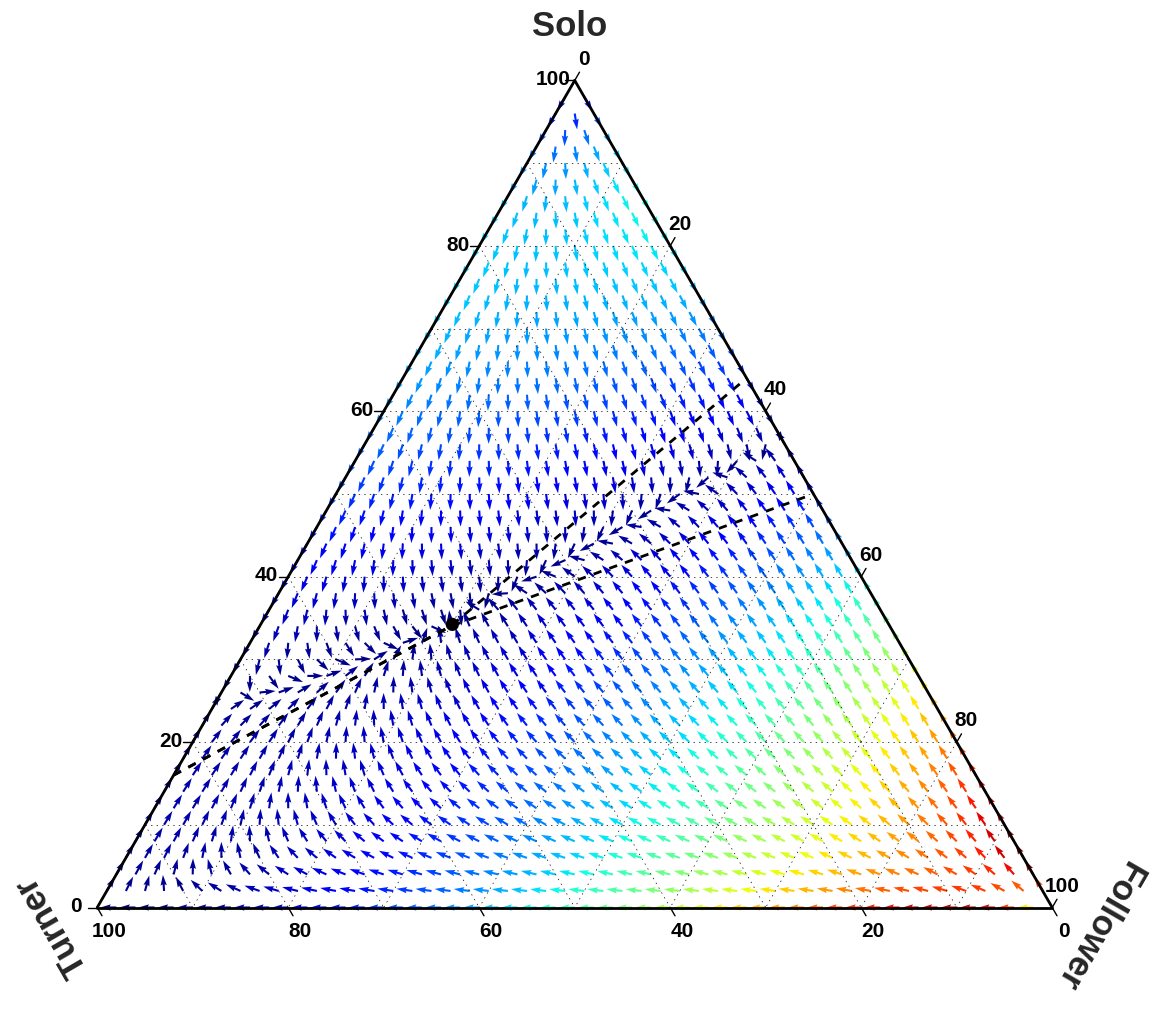
\includegraphics[scale=0.26]{fig/ArticleRob2/ExpectationsVectorsNormalized.png}}
          \end{subfigure}
          \begin{subfigure}[]
            {\label{fig:expectationsScatter} 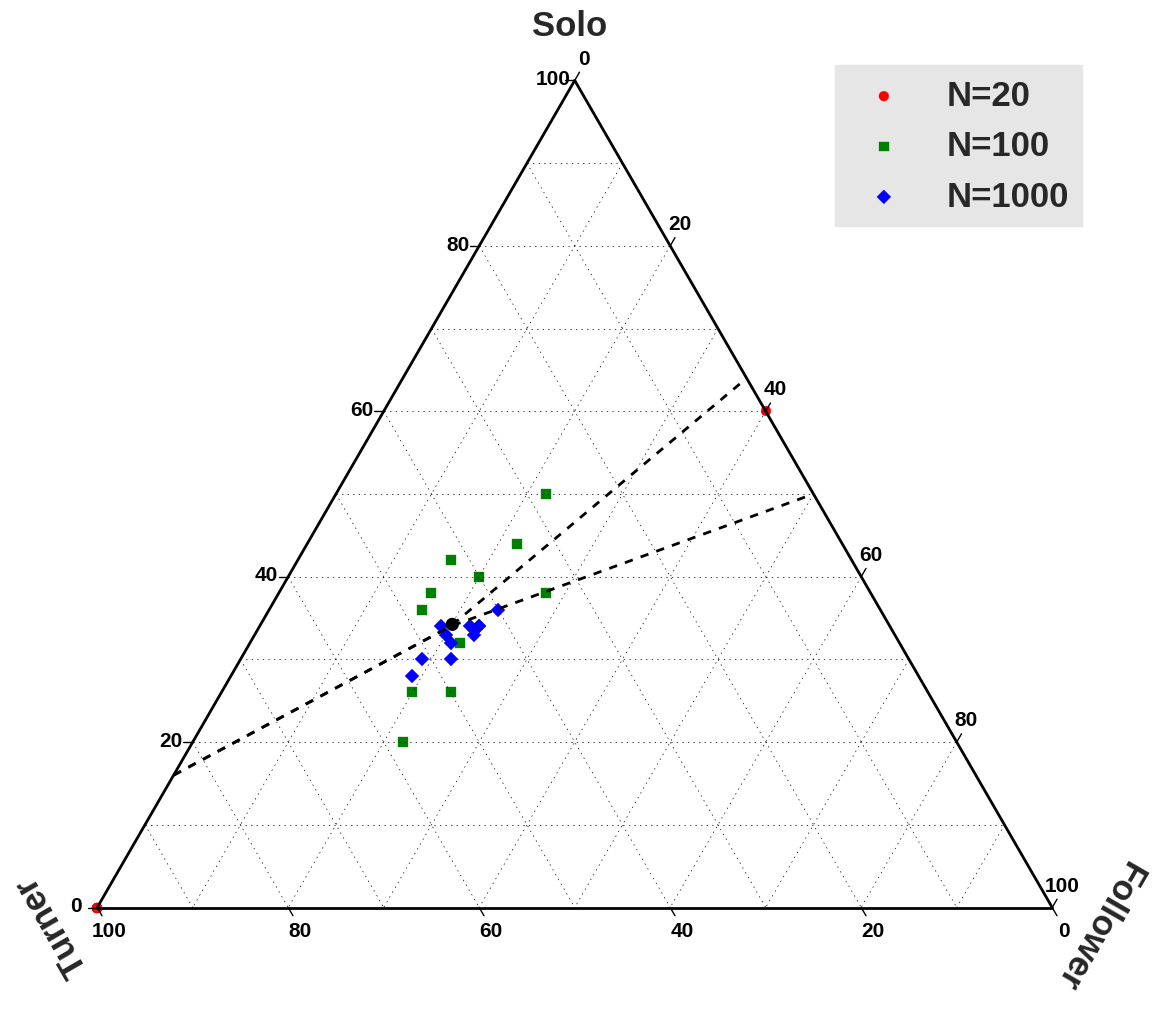
\includegraphics[scale=0.26]{fig/ArticleRob2/ExpectationsScatter.png}}
          \end{subfigure}
          \caption{\textbf{Vector field of the gradient of phenotypes' proportions and proportions of phenotypes at last generation of evolution.} {\em (a)}~Vector field of the gradient of phenotypes' proportions in an infinite population. The strength of variation is indicated by the color of the arrow. {\em (b)}~Repartition of phenotypes at the last generation of evolution for all three population sizes. Evolution lasted $1500$ generations and results were replicated across $11$ independent simulations. The initial population was entirely composed of \emph{solo} individuals.}
          \label{fig:ternary}
      \end{figure}

      Figure~\ref{fig:expectationsScatter} shows the final repartition of phenotypes after $1500$ generation of evolution for \(N=20\), \(N=100\) and \(N=1000\) in $11$ independent replicates. We can see that when increasing population size we also increase the probability that an equilibrium where the three phenotypes coexist is reached. We actually observe that the repartition of phenotypes at the last generation of evolution gets closer to the predicted equilibrium as population size increases. This implies that when population size increases, the effects of stochastic selection in a finite population decreases. Therefore the probability to lose particular phenotypes due to stochasticity is mitigated: population size is essential to the maintenance of specialists.


  \subsection{Key Properties for Evolving Heterogeneous Behaviours}

    From the previous Sections, we can deduce two key properties for the successful evolution of genotypic polymorphism. First, we showed that population size needs to be large enough in order to decrease the probability that heterogeneity could be lost during the evolutionary time. From this observation, we hypothesize that \textit{individuals need to be protected against the stochastic effects of selection}. Second, we previously saw that one key reason for the invasion of \emph{turner} individuals is that they perform quite well when paired together, even though they do not yield the best results. In other words, evolutionary dynamics does not necessarily lead to the best pairing in terms of performance, but to the most stable equilibrium between phenotypes.
  % while a pair of two \emph{followers} will perform badly and a pair with a \emph{solo} and a \emph{follower} fare better than any other. 
  From this observation, we hypothesize that \textit{the manner in which groups of interacting robots are formed is essential} for achieving an efficient specialisation.

    In order to test these hypotheses we design a last experiment where we diverge from the initial problem and now coevolve two separate populations. In this coevolution algorithm, each individual of one population is always evaluated against an individual of the other population ($5$ times as in previous experiments). Then, each population separately undergoes selection under an elitist \((10+10)\) selection method to create the population of the next generation (which means that each population's size is $20$). We conducted $11$ independent replicates which lasted $90000$ evaluations each. The populations were initially constituted of random individuals.

    \begin{table}[hbtp]
      \center{
        \begin{tabular}{cccc}
          \hline
          \textbf{\# L/F} & \textbf{\# Turning} & \textbf{\# NC} & \textbf{Total}\\ 
          \textbf{Strat.} & \textbf{Strat.} & \textbf{Strat.} & \\ 
          \hline
          11 & 0 & 0 & \textbf{11}\\
          \hline
        \end{tabular}
      }
      \caption{\textbf{Strategies evolved by the best individuals when coevolving two populations.} Repartition of the different strategies adopted by the best individuals at the last evaluation in each of the $11$ replicates. We indicate in each cell the number of simulations where a particular strategy evolved. Two populations were coevolved under elitist selection and the individuals' genotype values were initially random. In the table "L/F" stands for leader/follower and "NC" for "Non-Cooperative".}
      \label{tab:coevoStrategies}
    \end{table}

    We show (Table~\ref{tab:coevoStrategies}) that when using coevolution, we always evolve specialists in every replicates. Moreover, this algorithm is highly stable as the heterogeneous behaviours that emerged were never lost during evolution in every replicates. This means that coevolution is highly efficient both for the bootstrap of a leader/follower strategy and its maintenance throughout evolution. Regarding our hypotheses, we can check that the coevolution algorithm respects both of them. Firstly, as population are separatly coevolved, this algorithm is not sensible to the stochastic effects of small population size. Thus we ensure that the populations are highly protected against the disappearance of specialists. Secondly, we enforce a very specific pairing between individuals. Indeed individuals inside the same population are never partnered with one another. In this particular setup, this means that \emph{followers} end up being always paired with \emph{solo} individuals. As \emph{turners} then possesses no fitness benefit over the other phenotypes, their invasion will be prevented. The question is open as to how to endow an algorithm working on a single population with such properties.

  \subsection{Discussion and Conclusions}
  \label{sec:discussion}
    In this paper, we investigated the evolution of specialisation through a leader/follower strategy in a cooperative foraging task. Our goal was to reveal the difficulties that arise when trying to evolve genotypic polymorphism in a single population. To that end, we mainly studied the dynamics of evolution with two different selection methods: an \((\mu + \lambda)\) selection scheme and a fitness-proportionate selection scheme.

    We first showed that the long term evolution of a leader/follower strategy was nearly impossible with an elitist selection. However bootstrapping specialists was not a problem as we observed that they frequently emerged (and disappeared) during evolution. The major obstacle was rather to maintain heterogeneity over evolutionary time. Indeed, even when adding efficient \emph{followers} to a population of \emph{solo} individuals (i.e. \emph{leaders}) to force the adoption of a leader/follower strategy, specialists couldn't be maintained. In comparison, the properties shown by the fitness-proportionate algorithm were quite the opposite. While it was almost not capable of evolving a leader/follower strategy (nor any other cooperative strategy), the fitness-proportionate selection demonstrated high stability. It was therefore capable of maintaining specialists when present. We thus revealed two critical properties for evolving heterogeneous behaviours in a single population: \emph{bootstrapping} these behaviours and \emph{maintaining} them throughout evolution.

    We then ran computational analyses and showed that while a pair of \emph{turners} is indeed less efficient w.r.t. payoff than a pair of \emph{leader} and \emph{follower}, it is a lot more efficient than a pair of \emph{leaders} or a pair of \emph{followers}. As a result, these individuals can easily invade part of the population. Moreover, we also showed that the maintenance of specialists was very sensible to population size. Stochasticity in the selection process can indeed affect the stability of heterogeneity. Finally, a coevolution algorithm, which we showed to be always successful in evolving heterogeneous behaviours, solved both of these two problems with (1) \emph{specific partners selection} as pairs were constituted of individuals from different populations and (2) \emph{protection} of the behaviours evolved by applying selection separately on the two populations. While this coevolutionary algorithm is not capable (by design) of displaying genotypic polymorphism in a single population, it is sufficient to test and validate our hypotheses regarding the necessary properties for evolving efficient cooperative behaviours. Of course, the actual design of an algorithm using only one population to evolve heterogeneous individuals remains to be proposed.
    
    This raises several interesting perspectives on how to solve this problem. First, niche protection could prevent the disappearance of the efficient but unstable leader/follower strategy. As a matter of fact, coevolution is akin to a particular type of niches protection with $2$ niches. However, we intend to investigate how we could implement such mechanism without specifying the explicit number nor the organization of the niches. Rewarding diversity~\cite{Lehman2008} is also known as an effective way to protect novel behaviours and could be another promising direction. In particular, a multiobjective algorithm on performance and diversity~\cite{Doncieux2014}, by rewarding genotypic and phenotypic diversity, may protect evolved specialists.

    Secondly, we showed that because partners were chosen randomly among the population, it created the opportunity for a "parasitic" strategy to invade. An interesting direction for future work could be to investigate restrictions in the choice of partners. For example it would be compelling to investigate how the individuals could evolve to select their partner based on genotypic or phenotypic information.
  